\documentclass[12pt]{extreport} % Schriftgröße: 8pt, 9pt, 10pt, 11pt, 12pt, 14pt, 17pt oder 20pt

%% Packages
\usepackage{scrextend}
\usepackage{amssymb}
\usepackage{amsthm}
\usepackage{booktabs}
\usepackage{chngcntr}
\usepackage{cmap}
\usepackage{color}
\usepackage{csquotes}
\usepackage{enumitem}
\usepackage{float}
\usepackage{hyperref}
\usepackage{ulem}
\usepackage{lmodern}
\usepackage{makeidx}
\usepackage{amsmath}
\usepackage{mathtools}
\usepackage{xpatch}
\usepackage{pgfplots}
\pgfplotsset{compat=1.7}
\usetikzlibrary{calc}	
\usetikzlibrary{matrix}	

% Language Setup (English)
\usepackage[utf8]{inputenc} 
\usepackage[T1]{fontenc} 
\usepackage[english]{babel}

% Options
\makeatletter%%  
  % Linkfarbe, {0,0.35,0.35} für Türkis, {0,0,0} für Schwarz, {1,0,0} für Rot, {0,0,0.85} für Blau
  \definecolor{linkcolor}{rgb}{0,0.35,0.35}
  % Zeilenabstand für bessere Leserlichkeit
  \def\mystretch{1.2} 
  % Publisher definieren
  \newcommand\publishers[1]{\newcommand\@publishers{#1}} 
  % Enumerate im 1. Level: \alph für a), b), ...
  \renewcommand{\labelenumi}{\alph{enumi})} 
  % Enumerate im 2. Level: \roman für (i), (ii), ...
  \renewcommand{\labelenumii}{(\roman{enumii})}
  % Zeileneinrückung am Anfang des Absatzes
  \setlength{\parindent}{0pt} 
  % Für das Proof-Environment: 'Beweis:' anstatt 'Beweis.'
  \xpatchcmd{\proof}{\@addpunct{.}}{\@addpunct{:}}{}{} 
  % Nummerierung der Bilder, z.B.: Abbildung 4.1
  \@ifundefined{thechapter}{}{\def\thefigure{\thechapter.\arabic{figure}}} 
  % Chapter-Nummerierung beginnen bei (0):
  \setcounter{chapter}{0}
  % Chapter-Nummerierung
  \renewcommand\thechapter{\Roman{chapter}}
\makeatother%

% Meta Setup 
\title{Asset Pricing}
\author{Prof. Marliese Uhrig-Homburg}
\date{Sommersemester 2017}
\publishers{Karlsruher Institut für Technologie}

%% Math. Definitiones
\newcommand{\C}{\mathbb{C}}
\newcommand{\N}{\mathbb{N}}
\newcommand{\Q}{\mathbb{Q}}
\newcommand{\R}{\mathbb{R}}
\newcommand{\Z}{\mathbb{Z}}
\newcommand{\DO}[1]{\mathcal{D}\left( {#1} \right)}
\newcommand{\RO}[1]{\mathcal{R}\left( {#1} \right)}

\newtheoremstyle{named}{}{}{\normalfont}{}{\bfseries}{:}{0.25em}{#2 \thmnote{#3}}
\newtheoremstyle{nnamed}{}{}{\normalfont}{}{\bfseries}{:}{0.25em}{\thmnote{#3}}
\newtheoremstyle{itshape}{}{}{\itshape}{}{\bfseries}{:}{ }{}
\newtheoremstyle{normal}{}{}{\normalfont}{}{\bfseries}{:}{ }{}
\renewcommand*{\qed}{\hfill\ensuremath{\square}}

\theoremstyle{named}
\newtheorem{unnamedtheorem}{Theorem} \counterwithin{unnamedtheorem}{chapter}
\theoremstyle{nnamed}
\newtheorem*{unnamedtheorem*}{Theorem} 

\theoremstyle{itshape}
\newtheorem{definition}[unnamedtheorem]{Definition}

\theoremstyle{normal}
\newtheorem*{recall}{Recall}
\newtheorem*{example}{Example}
\newtheorem*{remark}{Remark}
\newtheorem*{satz}{Satz}
\newtheorem*{bemerkung}{Bemerkung}
\newtheorem*{beispiel}{Beispiel}


%% Template
\makeatletter%
\DeclareUnicodeCharacter{00A0}{ } \pgfplotsset{compat=1.7} \hypersetup{colorlinks,breaklinks, urlcolor=linkcolor, linkcolor=linkcolor, pdftitle=\@title, pdfauthor=\@author, pdfsubject=\@title, pdfcreator=\@publishers}\DeclareOption*{\PassOptionsToClass{\CurrentOption}{report}} \ProcessOptions \def\baselinestretch{\mystretch} \setlength{\oddsidemargin}{0.125in} \setlength{\evensidemargin}{0.125in} \setlength{\topmargin}{0.5in} \setlength{\textwidth}{6.25in} \setlength{\textheight}{8in} \addtolength{\topmargin}{-\headheight} \addtolength{\topmargin}{-\headsep} \def\pulldownheader{ \addtolength{\topmargin}{\headheight} \addtolength{\topmargin}{\headsep} \addtolength{\textheight}{-\headheight} \addtolength{\textheight}{-\headsep} } \def\pullupfooter{ \addtolength{\textheight}{-\footskip} } \def\ps@headings{\let\@mkboth\markboth \def\@oddfoot{} \def\@evenfoot{} \def\@oddhead{\hbox {}\sl \rightmark \hfil \rm\thepage} \def\chaptermark##1{\markright {\uppercase{\ifnum \c@secnumdepth >\m@ne \@chapapp\ \thechapter. \ \fi ##1}}} \pulldownheader } \def\ps@myheadings{\let\@mkboth\@gobbletwo \def\@oddfoot{} \def\@evenfoot{} \def\sectionmark##1{} \def\subsectionmark##1{}  \def\@evenhead{\rm \thepage\hfil\sl\leftmark\hbox {}} \def\@oddhead{\hbox{}\sl\rightmark \hfil \rm\thepage} \pulldownheader }	\def\chapter{\cleardoublepage  \thispagestyle{plain} \global\@topnum\z@ \@afterindentfalse \secdef\@chapter\@schapter} \def\@makeschapterhead#1{ {\parindent \z@ \raggedright \normalfont \interlinepenalty\@M \Huge \bfseries  #1\par\nobreak \vskip 40\p@ }} \newcommand{\indexsection}{chapter} \patchcmd{\@makechapterhead}{\vspace*{50\p@}}{}{}{}\def\Xint#1{\mathchoice
    {\XXint\displaystyle\textstyle{#1}} {\XXint\textstyle\scriptstyle{#1}} {\XXint\scriptstyle\scriptscriptstyle{#1}} {\XXint\scriptscriptstyle\scriptscriptstyle{#1}} \!\int} \def\XXint#1#2#3{{\setbox0=\hbox{$#1{#2#3}{\int}$} \vcenter{\hbox{$#2#3$}}\kern-.5\wd0}} \def\dashint{\Xint-} \def\Yint#1{\mathchoice {\YYint\displaystyle\textstyle{#1}} {\YYYint\textstyle\scriptscriptstyle{#1}} {}{} \!\int} \def\YYint#1#2#3{{\setbox0=\hbox{$#1{#2#3}{\int}$} \lower1ex\hbox{$#2#3$}\kern-.46\wd0}} \def\YYYint#1#2#3{{\setbox0=\hbox{$#1{#2#3}{\int}$}  \lower0.35ex\hbox{$#2#3$}\kern-.48\wd0}} \def\lowdashint{\Yint-} \def\Zint#1{\mathchoice {\ZZint\displaystyle\textstyle{#1}}{\ZZZint\textstyle\scriptscriptstyle{#1}} {}{} \!\int} \def\ZZint#1#2#3{{\setbox0=\hbox{$#1{#2#3}{\int}$}\raise1.15ex\hbox{$#2#3$}\kern-.57\wd0}} \def\ZZZint#1#2#3{{\setbox0=\hbox{$#1{#2#3}{\int}$} \raise0.85ex\hbox{$#2#3$}\kern-.53\wd0}} \def\highdashint{\Zint-} \DeclareRobustCommand*{\onlyattoc}[1]{} \newcommand*{\activateonlyattoc}{ \DeclareRobustCommand*{\onlyattoc}[1]{##1} } \AtBeginDocument{\addtocontents{toc} {\protect\activateonlyattoc}} \newcommand{\var}{\operatorname{var}} \newcommand{\cov}{\operatorname{cov}}\newcommand{\RightArrow}{\xRightarrow[]{ ~ ~ }} \newcommand{\LeftArrow}{\xLeftarrow[]{ ~ ~ }} \newcommand{\rightArrow}{\xrightarrow[]{ ~ ~ }} \newcommand{\leftArrow}{\xleftarrow[]{ ~ ~ }}
	% Titlepage
	\def\maketitle{ \begin{titlepage} 
			~\vspace{3cm} 
		\begin{center} {\Huge \@title} \end{center} 
	 		\vspace*{1cm} 
	 	\begin{center} {\large \@author} \end{center} 
	 	\vspace*{-0.5cm}
	 	\begin{center} \@date \end{center} 
	 		\vspace*{7cm} 
	 	\begin{center} \@publishers \end{center} 
	 		\vfill 
	\end{titlepage} }
\makeatother%

% Create Index
\makeindex 

\begin{document}

\pagenumbering{Alph}
\begin{titlepage}
	\maketitle
	\thispagestyle{empty}
\end{titlepage}

% Table of Contents
\tableofcontents
\thispagestyle{empty}

% Lecture Notes - Start 			
\pagenumbering{arabic}

\chapter{Einführung}

Es werden verschiedene Preise bzw. Renditen an Wertpapiermärkten betrachtet, unter anderem:

\begin{itemize}
	\item Aktienkurse
	\item Anleiherenditen
	\item Derivatenpreise
\end{itemize}

Warum stellen sich beobachtete Marktpreise bzw. Renditen ein? A priori bedeuten niedrige Price eine höhere Rendite. Man kann also die obige Frage auch umformulieren zu: warum einige Asset einen höheren erwarteten Return auszahlen als andere.

\subsubsection{Asset Pricing Theorie}
Es gibt zwei Aspekte die entscheidend in den Wert eines Assets einfließen. Einmal ist es die Verzögerung der Auszahlen, also wie lange man auf die Auszahlung des z.B. Wertpapiers warten muss und andererseits beeinflusst auch das zugrunde liegende Risiko den Wert des Assets. Auch wenn die Korrektur für die Verzögerung weniger problematisch ist, ist die Anpassung für das Risiko ein sehr viel wichtigerer Faktor für die Bewertung des Wertes eines Assets. Asset Pricing, wie viele anderer ökonomische Disziplinen, teilt den Zwiespalt in normativer zu deskriptiver Theorie. Asset Pricing liefert sowohl
\begin{itemize}
	\item Bewertungstheorien zur Erklärung der Preisbildung. Damit ist es möglich zu verstehen, warum sich Preise oder Returns so eingestellt haben, wie sie sind; als auch
	\item Schlussfolgerungen, falls Vorhersagen der Theorie $\neq$ Beobachtung. Was ein Verständnis dafür gibt, warum und wo Bewertungen sich falsch eingestellt haben und ggf. diese Schwächen ausnutzen.
	\item Ist eine Anpassung der Theorie erforderlich, so greift der Teil der positive Theorie an
\end{itemize}

Gerade der letzte Aspekt ist ein Grund für die Beliebtheit und vielzahligen praktischen Anwendung von Asset-Pricing. Denn eine \textbf{Fehlbewertung am Markt} ermöglicht eine \textbf{Handelsstrategie} (Normative Theorie). ~\bigskip

Diese auftretende Fehleinschätzung von Wertpapieren stammt unter anderem aus der oftmals vorherrschenden Asymmetrie von Informationen an einem Markt. Häufig sind keine Marktpreise für Ansprüche auf zukünftige Zahlungen vorhanden
\begin{itemize}
	\item geplante Investitionsprojekte
	\item Neuemissionen von Wertpapieren
	\item Finanzinnovationen
	\item $\dotsc$
\end{itemize}

Man findet demnach die Asset Pricing Theorie oft für zwei Grundlegende Aspekte:
\begin{itemize}
	\item zur Begründung, wie hoch fairer Preis sein sollte, und
	\item als wichtige Entscheidungsgrundlage
\end{itemize}

\section{Kernprinzipien der Finanzwirtschaft}
Bewertung fußt auf den Kernprinzipien der Finanzwirtschaft:
\begin{itemize}
	\item \textbf{Primat der Zahlungen}: für eine Entscheidung sind allein Zahlung (oder Zahlungsäquivalente) relevant; dies wird in der Literatur manchmal auch als \textit{Dominance} bezeichnet.
	\item \textbf{Zeitwert des Geldes}: der Wert einer Zahlung hängt davon ab, wann sie erfolgt
	\item \textbf{Ertrag vs. Risiko}: bei vielen Entscheidungen ist eine Abwägung zwischen Ertrag und Risiko zu treffen.
	\item \textbf{Aggregation durch Märkte}: Wertpapiermärkte aggregieren Präferenzen und Informationen
	\item \textbf{Arbitragefreiheit}: Preise an kompetativen Wertpapiermärkten zeichnen sich durch die Abwesenheit von Arbitrage aus
\end{itemize}

\section{Relative vs. absolute Bewertung}
Es gibt zwei teilweise gegenläufige Ansätze zur Bewertung von Assets
\begin{description}
	\item \textbf{absolut}: mit Bezug zu grundlegenden makroökonomischen Faktoren.
		\begin{itemize}
			\item Konsum-basierte oder allgemeine Gleichgewichtsmodelle
			\item Beispiel: capital Asset Pricing Model
		\end{itemize}
	\item \textbf{relativ}: zu gegebenen anderen Wertpapieren (Basiswertpapieren)
		\begin{itemize}
			\item Duplikation und Gesetz des einen Preises
			\item Beispiel: Optionspreistheorie nach Black/Scholes
		\end{itemize}
\end{description}
Typische Anwendungen enthalten beide Aspekte und der Anteil zu welchem man den einen oder anderen Ansatz  wählt, hängt für gewöhnlich vom betrachteten Asset und Grund für die Bewertung ab.

\section{Bewertungsprinzip}
Asset Pricing liegt eine einfach Grundidee zugrunde:
$$ \textit{Preise entsprechen erwarteten diskontierten Zahlungen} $$ 

\textbf{Zahlungsstrom}: Zukünftige unsichere Zahlungen müssen aufgrund deren Zeit- und Risikodimension bewertet werden. Unser Bewertungsprinzip berücksichtigt diese Dimensionen durch geeignete
\begin{itemize}
	\item Diskontierung
	\item Erwartungsbildung
\end{itemize}

\chapter{Stochastischer Diskont-Faktor Ansatz}

\enquote{Asset pricing theory all stems from one simple concept, presented in the first page of the first chapter of this book: \textbf{price equals expected discounted payoff}. The rest is elaboration, special cases, and a closet full of tricks that make the central equation useful from one or another application.} ~\\ 
	\begin{tabular}{lr} ~\\
  		\hspace{6.35cm} & \textit{Quelle: John H. Cochrane, Asset Pricing, S. xiii}
	\end{tabular} ~\\ ~\bigskip

Bei einem gegebenen Zahlungsstrom (z.B. Dividenden, Zinsen, Auszahlungen von Derivaten, Rückflüsse aus Investitionen, $\dotsc$) ergeben sich für uns die folgenden Fragestellungen: 
\begin{itemize}
	\item Welchen Wert besitzt der Zahlungsstrom?
	\item Wie wirken sich Zeit und Risiko auf den Wert aus?
	\item Wie ändert sich Wert, wenn sich Ökonomie verändert? (Risikomanagement)
\end{itemize}
~\\
Wir betrachten dies in einem einfachen formaler Rahmen:
\begin{itemize}
	\item gegeben: zukünftige (unsichere) Zahlung $x_{t+1}$
	\item gesucht: Heutiger Wert $p_t$
\end{itemize}

~\newpage

\section{Präferenzen der Investoren}

Zinsrate korrelieren mit dem erwarteten marginalen Nutzenwachstum, denn es macht Sinn z.B. bei hohen Zinsen möglichen Konsum auszusetzen und zu sparen, in Bonds zu investieren und den Konsum auf die Zukunft zu verschieben. Die Risikokorrektur des Wertes eines Assets sollte außerdem von der Kovarianz der Auszahlung mit den marginalen Nutzen bzw. Konsum zusammenhängen, denn ein Asset welches in ökonomisch schlechteren Zeiten mehr auszahlt wird besser bewertet, als eins welches auf ökonomisch gute Zeiten baut. ~\\

Hier ist marginaler Nutzen, und nicht Konsum, das grundlegende Maß für die Einstellung von Nutzern. Betrachtet man unter anderem das Konsumlevel eines Nutzers, so sieht man, dass dies niedrig sein kann, wenn der marginale Nutzen hoch ist. Also könnte man davon ausgehen, dass der Konsum als Indikator für den marginalen Nutzen verwendet werden kann. Das Konsumlevel ist auch niedrig, und in diesem fall der marginale Nutzen auch hoch, wenn die anderen Assets des Investors schlecht performen. Aus diesem Grund gehen wir davon aus, dass die Preise von Assets die eine positive Kovarianz mit einem Marktindex besitzen niedrig ist. ~\\


Also fangen wir mit der grundlegenden Idee an: der Investor trifft wirtschaftliche Entscheidungen mit dem Ziel, möglichst günstigen Konsumstrom zu erreichen. Formal erfolgt dies über die Nutzenfunktionen (additiv und separabel):
	$$ U(c_t, c_{t+1}) = u(c_t) + \beta \cdot \mathbb{E}_t\left[ u\left(c_{t+1}\right) \right], $$
wobei $c_t =$ Konsum in $t$ und $c_{t+1} =$ Konsum in $t+1$ beschreibt. $\beta$ stellt den subjektiven Diskontfaktor dar, denn im Allgemeinen ist es relevant, wann die Zahlung stattfindet; man kann sich dies auch als einen ungeduldigen Investor vorstellen. Der Erwartungswert muss gebildet werden, da der Konsum in $t+1$ unsicher und damit eine Zufallsvariable ist. 

\newpage

Plausible Annahmen bezüglich der Eigenschaften von solchen Nutzenfunktionen wären
\begin{itemize}
	\item \textbf{positiver Grenznutzen} ($u' > 0$): Nutzen wächst, wenn Konsum in beliebigem Zeitpunkt wächst, d.h. \enquote{mehr ist besser als weniger} (nicht gesättigte Investoren)
	\item \textbf{abnehmender Grenznutzen} ($u'' < 0$): Je höher der Konsum in einem Zeitpunkt, desto geringer ist der durch zusätzliche Konsumeinheit erzeugte Nutzenzuwachs
\end{itemize} 

\begin{figure*}[h!] \centering
	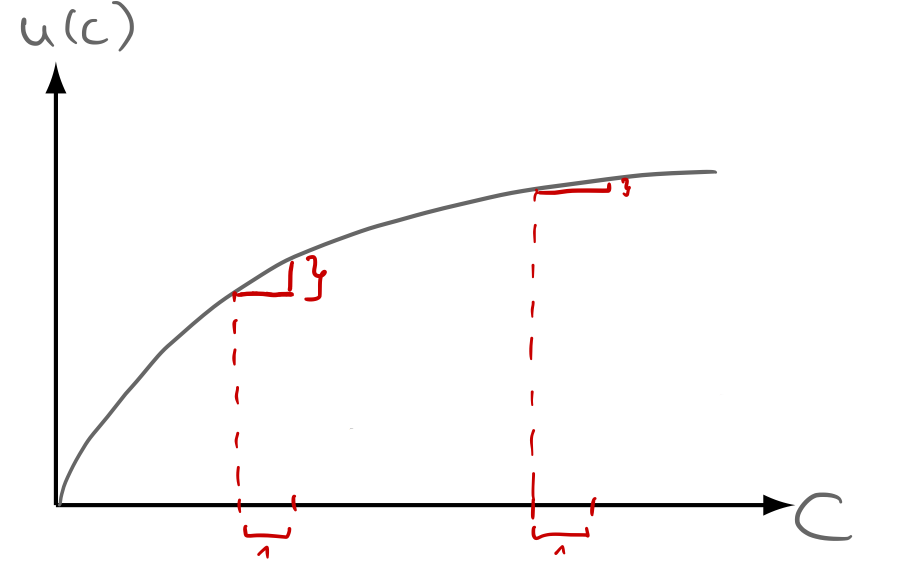
\includegraphics[scale=0.2725]{img/p17}
\end{figure*}

Die Nutzenfunktion bildet Ungeduld und Risikoaversion der Investoren ab:

\begin{itemize}
	\item \textbf{Ungeduld}: $\beta < 1$ erfasst Präferenz für frühere Zahlungen subjektive Diskontierung
	\item \textbf{Risikoaversion}: zukünftiger Konsum $c_{t+1}$ ist unsicher, daher muss bei dessen Nutzen der Erwartungswert $\mathbb{E}_t \big[ u(c_{t+1}) \big]$ betrachtet werden. Hierbei ist die Krümmung der Nutzenfunktion $u$ zentral, wie im folgenden Beispiel verdeutlich wird.
\end{itemize} 

\begin{beispiel}[50/50 Wette] ~\\
	Für einen Nutzer sei mit Wahrscheinlichkeit $0.5$ höher $\overline{c} + x$ oder niedriger $\overline{c} - x$ Konsum zu erwarten. Der Nutzen aus dieser unsicheren Situation ergibt sich damit zu
		$$ \mathbb{E} \big[ u(c) \big] = 0.5 \cdot u ( \overline{c} + x ) + 0.5 \cdot u ( \overline{c} - x ). $$
	Da die Nutzenfunktion $u$ konkav ist, würde der Investor die Wette meiden, da $\mathbb{E}\left[ u\left(c + X\right) \right] < u\left(\mathbb{E}\left[c+ X\right]\right)  = u \left( \overline{c} \right)$.
\end{beispiel} 

\begin{figure*}[h!] \centering
	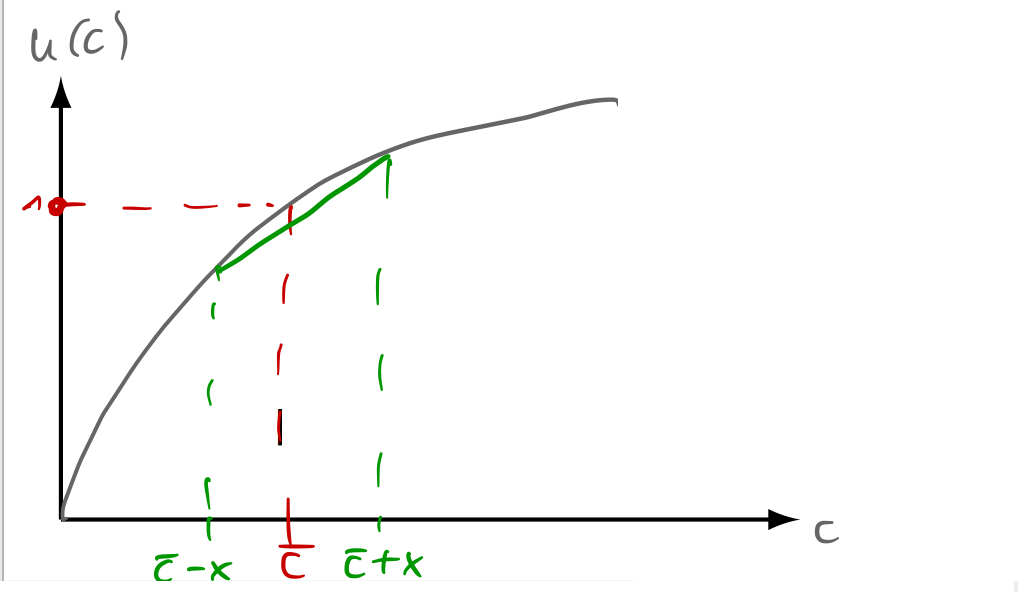
\includegraphics[scale=0.2725]{img/p18}
\end{figure*}

~\newpage

Der Gesamtnutzenfunktion $U(c_t, c_{t+1})$ ist am einfachsten über Nutzenindifferenzkurven darstellbar (streng konvex, da abnehmender Grenznutzen; linear, wenn keine Risikoaversion vorliegt): 
\begin{figure*}[h!] \centering
	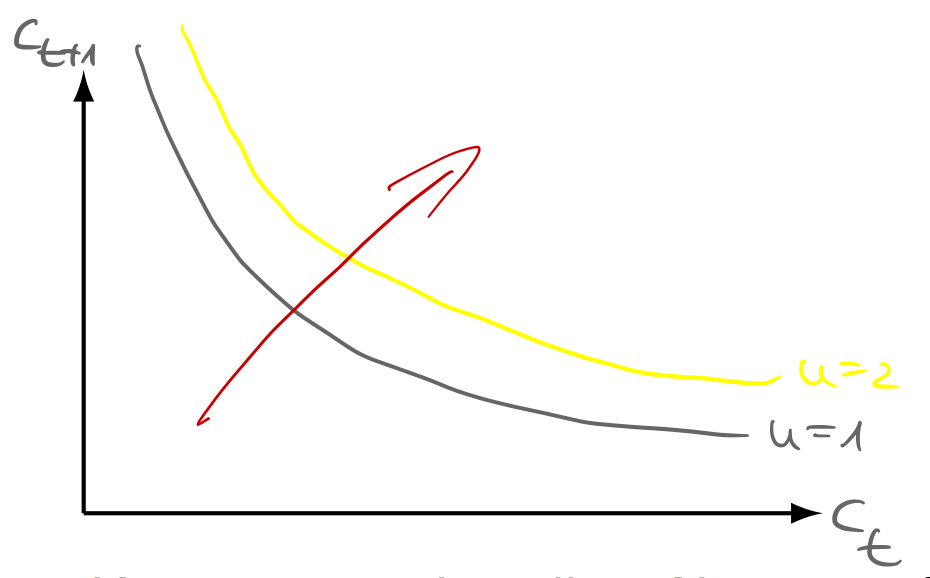
\includegraphics[scale=0.4]{img/p19}
\end{figure*}

\begin{itemize}
	\item Alle Punkte auf einer Kurve weisen denselben Nutzen auf.
	\item Je weiter entfernt vom Ursprung, desto höher der Nutzen $\rightarrow$ folgt aus positivem Grenznutzen
	\item Iso-Nutzenlinien verlaufen (streng) konvex. $\rightarrow$ folgt aus abnehmendem Grenznutzen
	\item Aversion gegen intertemporale Substitution
\end{itemize}

~\newpage

\section{Beispiele für Nutzenfunktionen}
Zwei zentrale Beispiele für Nutzenfuntionen, die die obigen Anforderungen erfüllen sind:
\begin{itemize}
	\item \textbf{Power-Nutzenfunktion}
			$$ u(c) = \frac{c^{1-\gamma} - 1}{1 - \gamma} $$
			Für diese Nutzenfunktion gilt:
		\begin{itemize}
			\item die Ableitungen sind
				\begin{align*}
					u' & = c^{-\gamma} > 0 \\
					u'' & = - \gamma \cdot c ^{-\gamma - 1} < 0
				\end{align*}
			\item somit ist
				$$- c \cdot \frac{u''(c)}{u'(c)} = \gamma, $$
				d.h. es liegt eine konstante relative Risikoaversion vor.
			\item sie streben für $\gamma \rightarrow 1$ gegen Log-Nutzenfunktion
		$$ u(c) = \ln(c) $$
		\end{itemize}
	\item \textbf{Quadratische Nutzenfunktion}
			$$ u(c) = - \frac{1}{2} \left( \overline{c} - c \right)^2, \quad c < \overline{c} $$
			\begin{figure*}[h!] \centering
				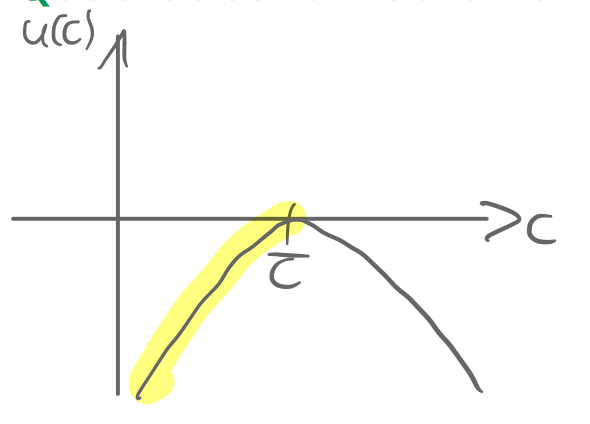
\includegraphics[scale=0.4]{img/p20}
			\end{figure*}
\end{itemize}

~\newpage

\section{Zentrale Bewertungsbeziehung}

Ein Investor konsumiert in den zwei betrachteten Perioden $c_t, c_{t+1}$ und kann einen beliebigen Anteil $\xi$ der Zahlung $x_{t+1}$ kaufen oder verkaufen. Seien $e_t$, $e_{t+1}$ die Ausgangslevel an Konsum die der Investor ohne $x$ kaufen würden, z.B. festes Einkommenslevel vor Investitionen. Das Kalkül des Investors lautet dann:
		$$ \max_{\xi} u(c_t) + \beta \mathbb{E}_t \big[ u(c_{t+1}) \big] $$
	unter den Nebenbedingungen: 
		\begin{align*}
			c_{t} & = e_t - p_t \xi \\
			c_{t+1} & = e_{t+1} + x_{t+1} \xi
		\end{align*}
Durch Einsetzen der Nebenbedingungen, liefert Bedingung erster Ordnung für $\xi$ damit:
	$$ p_t u'(c_t) = \mathbb{E}_t \big[ \beta u'(c_{t+1}) x_{t+1} \big] $$
Diese Gleichung stellt die gewöhnliche marginale Bedingung für ein Opzimum dar: $p u'(c_t)$ ist der Verlust des Nutzens den ein Investor trägt falls er eine weitere Einheit kauft; $\mathbb{E}_t \big[ \beta u'(c_{t+1}) x_{t+1} \big]$ ist der Zuwachs in diskontiertem, erwartetem Nutzen den der Investor von einem zusätzlichen Payoff in $t+1$ erhält. Die Bedinung erster Ordnung stellt also das Gleichgewicht dar, indem der Investor so lange kauft oder verkauft bis die Grenzkosten  gleich dem erwarteten Grenzertrag gleicht. ~\\

Aus der first-order Bedingung folgt durch Umformung die zentrale Bewertungsgleichung
	$$ p_t = \mathbb{E}_t \big[ \beta \frac{u'(c_{t+1})}{u'(c_t)} x_{t+1} \big], $$
welche in vielen Fällen hilfreich ist, obgleich sowohl \textbf{Preis} als auch \textbf{Konsum} endogene Größen sind. 

~\newpage

\section{Stochastischer Diskontfaktor}

Wir teilen obige Gleichung des einfachen konsumbasierten Modells auf um folgende hilfreiche Separation zu erhalten:

\begin{itemize}
	\item Mit stochastischem Diskontfaktor
	 $$ m_{t+1} = \beta \frac{u'(c_{t+1})}{u'(c_t)} $$
	\item vereinfacht sich zentrale Bewertungsbeziehung zu
	 $$ p_t = \mathbb{E}_t \big[ m_{t+1} x_{t+1} \big] $$
\end{itemize}

Stochastische Diskontfaktor verallgemeinert übliches Verständnis von Diskontfaktoren:

\begin{itemize}
	\item Bei einer sicheren Zahlung $x_{t+1}$, sei $R^f = 1 + r^f$ der risikolose Brutto-Zinssatz und so ergibt sich der Zusammenhang: $$p_t = \frac{1}{R^f} x_{t+1} = \frac{1}{1+r^f} x_{t+1}$$
	\item Risikobelastete Zahlungen können mit einer risikoadjustierte Diskontierung behandelt werden. Sei $R^i$ der risiko-angepasste, asset-spezifische Diskonfaktor, so ergibt sich: $$p_t = \frac{1}{\mathbb{E} \left[R^i \right]} \mathbb{E}_t \big[ x_{t+1}^i \big]$$
\end{itemize}

Beachte dass aufgrund der Diskontierung und des Bildens des Erwartungswertes, dass in first-order Bedingung nur ein Diskontfaktor $m$ vorkam, unabhängig vom möglichen Risiko oder betrachteten Asset, d.h. der stochastische Diskontfaktor $m_{t+1}$
\begin{itemize}
	\item ist zufällig, was in der Literatur auch stochastisch genannt wird, und
	\item für alle Assets (bzw. Cash Flows $x_{t+1}$) identisch.
\end{itemize}
Wie passt das mit der üblichen Vorstellung zusammen, dass riskantere Titel eine höhere Diskontierung erfordern? Die Korrelation zwischen den zufälligen Teilen des Dikontfaktors $m$ und asset-spezifischen Payoffs $x^i$ korrigiert für das asset-spezifische Risiko. Neben bei, es gibt verschiedene Interpretationen und alternative Bezeichnungen für $m_{t+1}$, z.B.:
\begin{itemize}
	\item Grenzrate der Substitution: $m_{t+1} = \beta \frac{u'(c_{t+1})}{u'(c_t)}$
	\item Pricing Kernel, Dichte der Zustandspreise
\end{itemize}

~\newpage

\section{Beispiele für Preise und Zahlungen}

\begin{itemize}
	\item \textbf{Aktieninvestment}: $p_t$: Preis in $t$, $x_{t+1} = p_{t+1} + d_{t+1}$: Zahlung in $t+1$ mit Dividendenzahlung $d_{t+1}$ in $t+1$ (geschickter: Returns nehmen, statt stationär):
		$$ p_t = \mathbb{E}_t \big[ m ( p_{t+1} + d_{t+1} ) \big] $$
	\item \textbf{Brutto-Return}: Interpretiere $R_{t+1} = \frac{x_{t+1}}{p_t}$ als Payoff in $t + 1$ mit Preis 1 dann gilt (mit $m$ als stoch. Diskontfaktor)
		$$ 1 = \mathbb{E}_t \big[ mR \big] $$
	\item \textbf{Überschuss-Return}: als Zahlung $R_{t+1}^e = R_{t+1}^a - R_{t+1}^b$ in $t + 1$ eines Portfolios ohne Kapitaleinsatz, d.h. $p_t = 0$ dann gilt (beachte: Arbitrage-Portfolio, da kein Kapitaleinsatz)
			$$ 0 = \mathbb{E}_t \big[ mR^e \big] \quad 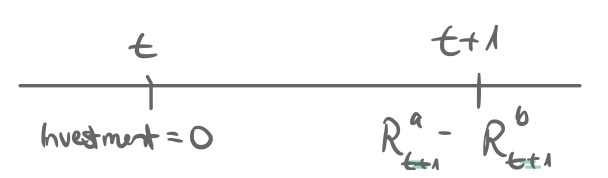
\includegraphics[scale=0.275]{img/p25} $$
	\item \textbf{Einperiodige Anleihe}: $p_t$: Anleihepreis in $t$, Rückzahlung (risikolos) $x_{t+1} = 1$: 
			$$ p_t = \mathbb{E}_t \big[ m \big] \quad 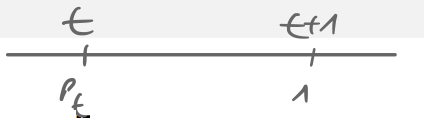
\includegraphics[scale=0.275]{img/p26-1} $$
		(d.h. Diskontfaktor (bei sicheren Zahlungen) $\hat{=}$ erwarteter stoch. Diskontfaktor)
	\item \textbf{Geldmarktkonto}: $p_t = 1$, Rückfluss in $t + 1$: $R^f = (1 + r^f)$ dann gilt:
		 $$ 1 = \mathbb{E}_t \big[ mR^f \big] \quad 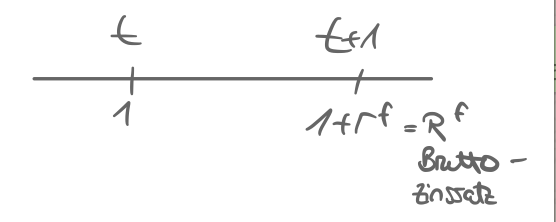
\includegraphics[scale=0.275]{img/p26-2} $$

	\item \textbf{Kaufoption}: $p_t = C$, $x_{t+1} = \max(S_{t+1} - K, 0)$, dann gilt: 
		$$ C = \mathbb{E}_t \big[ m \left( \max ( S_{t+1} - K, 0 ) \right) \big] \quad 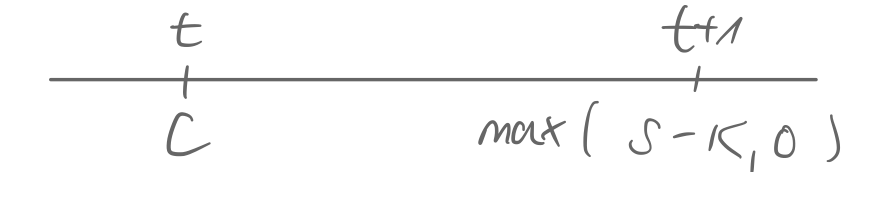
\includegraphics[scale=0.275]{img/p26-3} $$
\end{itemize}

\chapter{Klassische Theorien}

Durch einfache Umformungen der zentralen Bewertungsbeziehung
$$ p = \mathbb{E}[mx] $$
lassen sich viele finanzwirtschaftliche Theorien und Konzepte leicht ableiten, z.B.:
\begin{enumerate}[label=\arabic*\upshape.]
	\item \textbf{Ökonomie der Zinsen}: Wann und warum sind Zinsen hoch oder niedrig?
	\item \textbf{Risikoanpassung}: Wovon hängt die Risikoanpassung ab?
	\item \textbf{Unsystematisches Risiko}: Warum wird unsystematisches Risiko nicht vergütet?
	\item \textbf{Beta als Risikomaß}: Welche Beziehung besteht zwischen erwarteten Renditen und Beta?
	\item \textbf{$\mu$-$\sigma$-Rand}: Welche Rendite/Risiko-Kombinationen sind erreichbar?
	\item \textbf{Equity Premium Puzzle}: Warum sind Risikoprämien von Aktien so hoch?
\end{enumerate}

~\newpage

\section{Ökonomie der Zinsen}

Interpretation der risikolosen Verzinsung $R^f = 1 + r^f$.
\begin{itemize}
	\item Aus der zentralen Bewertungsbeziehung folgt für das Geldmarktkonto:
		$$ 1 = \mathbb{E} \left[ m R^f \right] \Rightarrow R^f = \frac{1}{\mathbb{E}[m]} $$
	\item Bei Sicherheit folgt für eine isoelastische Nutzenfunktion
		$$ u(c) = \frac{c^{1-\gamma} - 1}{1 - \gamma}: ~ m_{t+1} = \beta \frac{u'(c_{t+1})}{u'(c_{t})} = \beta \left( \frac{c_{t+1}}{c_t} \right)^{-\gamma} $$
		$$ \Rightarrow R^f = \frac{1}{\beta} \left( \frac{c_{t+1}}{c_t} \right)^{\gamma} $$
	\item Somit gilt:
		\begin{itemize}
			\item Realzinsen sind hoch, wenn Investoren ungeduldig sind (niedriges $\beta$)
			\item Realzinsen sind hoch, wenn das Konsumwachstum hoch ist.
			\item Realzinsen reagieren sensitiver auf Änderungen des Konsumwachstums bei hoher Riskoaversion (hohes $\gamma$).
		\end{itemize}
\end{itemize}
	
	
\begin{figure*}[h!] \centering
	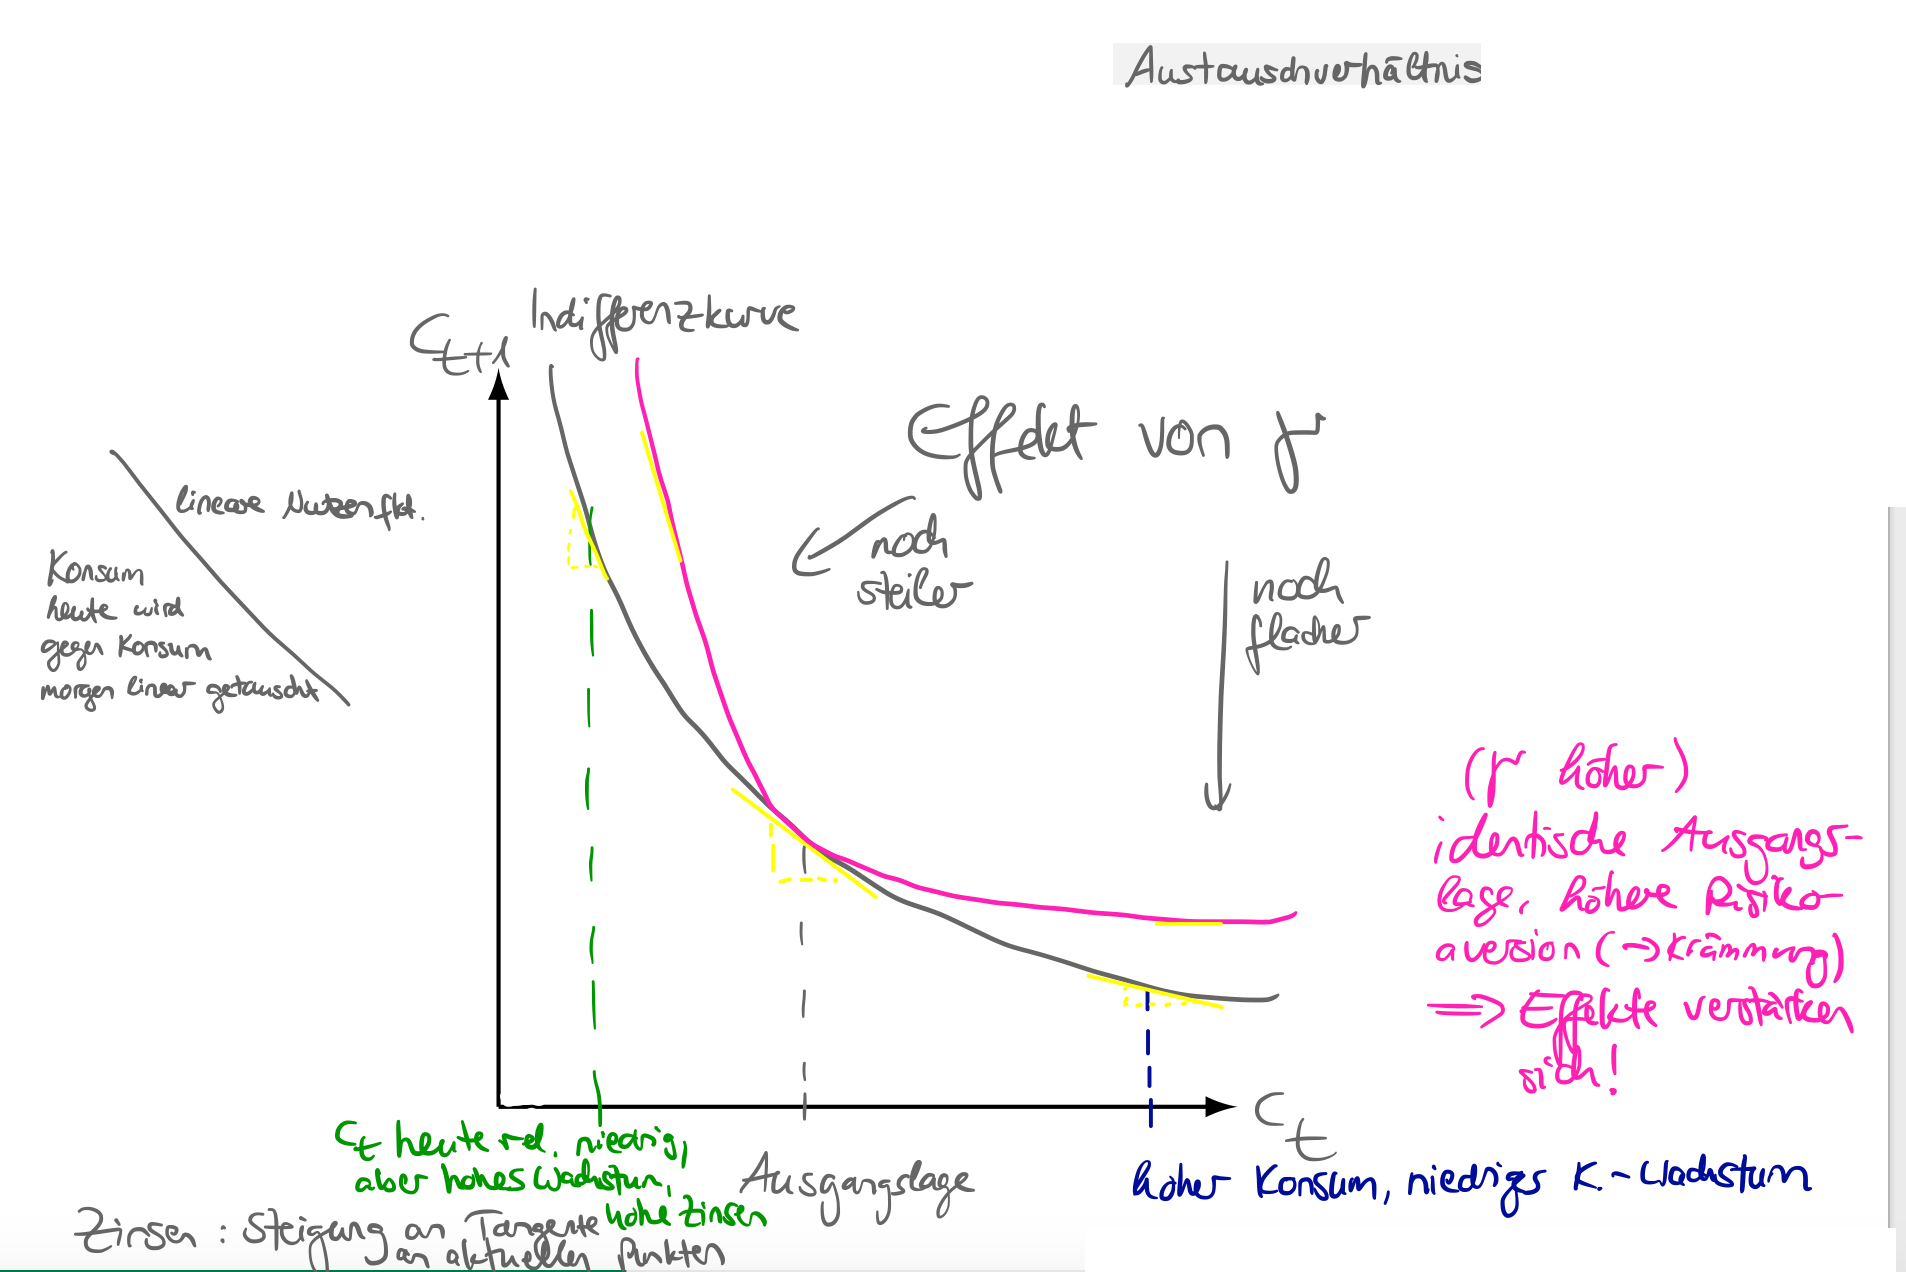
\includegraphics[scale=0.2725]{img/p29}
\end{figure*}

	
Unter Annahme von Unsicherheit:	
\begin{itemize}
	\item Mit $\beta = e^{-\delta}$ und $\Delta c_{t+1} = \ln \left( \frac{c_{t+1}}{c_t} \right)$ folgt
		$$ m_{t+1} = e^{-\delta} e^{-\gamma \Delta c_{t+1}} \approx 1 - \delta - \gamma \Delta c_{t+1} $$
	\item Somit
		$$ R^f = \frac{1}{\mathbb{E}[m_{t+1}]} \approx \frac{1}{1 - \delta - \gamma \mathbb{E}_t[\Delta c_{t+1}]} \approx 1 + \delta + \gamma \mathbb{E}[\Delta c_{t+1}] $$
	\item Grundsätzlich identische Implikationen wie im deterministischen Fall:
		$$ R^f \approx 1 + \delta + \gamma \mathbb{E} [\Delta c_{t+1}] $$
\end{itemize}
Wie schon zuvor sind Zinsen hoch
\begin{itemize}
			\item bei sehr ungeduldigen Investoren (niedriges $\beta$ bzw. hohes $\delta$)
			\item bei hohem erwarteten Konsumwachstum $\mathbb{E}_t[\Delta c_{t+1}]$
				\begin{itemize}
					\item wer weiß, dass er in Zukunft reicher sein wird, braucht hohe Zinsen, damit er bereit ist, heute auf Konsum zu verzichten und dafür zu sparen
					\item Zinsen sind höher in Aufschwungphasen als in Rezessionen
				\end{itemize}
\end{itemize}
Wie schon zuvor
\begin{itemize}
	\item Sensitivität bzgl. Konsumwachstum nimmt mit Risikoaversion $\gamma$ zu
		\begin{itemize}
			\item Beachte: hohes $\mathbb{E}_t[\Delta c_{t+1}]$ (Aufschwung), hohes $R^f$; ~\\
				niedriges $\mathbb{E}_t[\Delta c_{t+1}]$ (Abschwung), niedriges $R^f$;
			\item Stärke der Veränderung (ob positiv  oder negativ) steigt mit $\gamma$
		\end{itemize}
\end{itemize}

Nun zum Aspekt des Risikos. Betrachte hierzu Approximation zweiter Ordnung:
	$$	R^f \approx 1 + \delta + \gamma \mathbb{E}_t[\Delta c_{t+1}] - \frac{1}{2} \gamma^2 \sigma^2_t (\Delta c_{t+1}) $$ 
	
~\newpage

Höhere Volatilität des Konsumwachstums (hohes $\sigma$)
\begin{itemize}
	\item führt zu niedrigeren Zinsen
		\begin{itemize}
			\item in unsicheren Zeiten spart man lieber vorsorglich (precautionary savings)
			\item hohe Sparnachfrage reduziert Zinsen % todo stimmt das? Was sind sparnachfragen?
		\end{itemize}
\end{itemize}

Umgekehrt
\begin{itemize}
	\item ist Konsumwachstum hoch, falls Zinsen hoch sind (bei hohen Zinsen wird mehr gespart)
	\item ist Konsum weniger sensitiv bzgl. Zinsänderungen, wenn $\gamma$ hoch ist (hohes $\gamma \Rightarrow$ starker Wunsch nach gleichmäßigem Konsumstrom)
\end{itemize}

Was determiniert wen?
\begin{itemize}
	\item Konsum determiniert Zinsen (vgl. geschlossene Volkswirtschaft, Gesamtökonomie)
	\item Zinsen determinieren Konsum (siehe Analysten, Eizelpersonen)
\end{itemize}

Beachte, dass bei der Power-Nutzenfunktion gilt, dass der Krümmungsparameter $\gamma$ gleichzeitig die folgenden Aspekte steuert:
\begin{itemize}
	\item \textbf{intertemporale Substitution}: Aversion gegenüber zeitlich schwankenden Konsummöglichkeiten
	\item \textbf{Risikoaversion}: Aversion gegenüber Veränderungen der Konsummöglichkeiten durch unterschiedliche Zustände
	\item \textbf{vorsorgliche Ersparnis}: abhängig von der dritten Ableitung der Nutzenfunktion
\end{itemize}
 Allgemeinere Nutzenfunktionen entkoppeln die drei Einflüsse. Beispiel: ~ Rekursive Nutzenfunktion (Epstein-Zin Nutzenfunktion, siehe z.B. RRA (relative risk aversion), IES (intertemporal elasticity of substitution)). 

~\newpage

\section{Risikoanpassung}

\begin{itemize}
	\item Aus der Definition $\cov(m,x) = \mathbb{E}[mx] -  \mathbb{E}[m]  \mathbb{E}[x]$ folgt
		$$ p =  \mathbb{E}[mx] =  \mathbb{E}[m] \mathbb{E}[x] - \cov(m, x) $$
	\item Mit $R^f = \frac{1}{\mathbb{E}[m]}$ folgt
		$$ p = \frac{\mathbb{E}[x]}{R^f} + \cov(m, x) $$
\end{itemize}

d.h. je höher die Kovarianz desto höher ist der Preis; wir haben somit eine Risikokorrektur über die Kovarianz. Der Preis ergibt sich aus
\begin{itemize}
	\item Diskontierung des erwarteten Payoffs mit risikolosem Zinssatz
		\begin{itemize}
			\item Standardbarwert-Kalkül bei Sicherheit bzw. Risikoneutralität
			\item Aspekt \enquote{Zeit}, beachte dass 
			\begin{itemize}
				\item unter Sicherheit die Kovarianz gleich 0 ist, da $x$ unter Sicherheit eine Konstante ist, und 
				\item unter Risikoneutralität fällt die Kovarianz ebenfalls weg, da $m$  konstant ist, da die Nutzenfunktionen linear sin, und somit die Steigung bzw. $u'(c_{t+1})$ konstant ist und somit der Nenner konstant ist.
			\end{itemize} 
		\end{itemize}
	\item Risikokorrektur erfolgt über den Kovarianzterm
		\begin{itemize}
			\item je stärker Kovarianz mit Diskontfaktor $m$, desto höher der Preis
			\item Aspekt \enquote{Risiko}
		\end{itemize}
\end{itemize}

~\newpage

\subsubsection{Wirkungsweise der Risikoanpassung}

Mit dem Diskontfaktor $m = \beta \frac{u'(c_{t+1})}{u'(c_t)}$ folgt
	$$	p = \frac{\mathbb{E}[x]}{R^f} + \frac{\cov(\beta u'(c_{t+1}), x_{t+1})}{u'(c_t)} $$
Risikoanpassung
\begin{itemize}
	\item verringert Preis bei positiver Kovarianz mit Konsum ($u'(c)$ sinkt in $c$)
	\item erhöht Preis bei negativer Kovarianz mit Konsum
\end{itemize}
Warum?

\begin{beispiel}
	Betrachte zwei Wertpapiere mit 
	
	\begin{figure*}[h!] \centering
		\begin{tabular}{l|cc}
  			~  & gute Zeiten (0.5) & schlechte Zeiten (0.5) \\
  			\hline
 			$WP_1$ & $100$ & $0$ \\
  			$WP_2$ & $0$ & $100$
		\end{tabular}
	\end{figure*} 

	Für welches Wertpapier sind Sie bereit mehr zu bezahlen?	
\end{beispiel}


Ergebnis:
\begin{itemize}
	\item Für Assets, die mehr zur Konsumglättung beitragen (hier WP2), werden höhere Preise bezahlt.
	\item Bei unsicherem Payoff mit gegebenem Erwartungswert $\mathbb{E}[x]$
		\begin{itemize}
			\item wird Preis nach unten korrigiert, falls Payoff in schlechten Zeiten niedrig ist
			\item wird Preis nach oben korrigiert, falls Payoff in schlechten Zeiten hoch ist (Versicherungsidee)
		\end{itemize}
\end{itemize}

Rolle der Risikoaversion
\begin{itemize}
	\item Betrachte wieder isoelastische Nutzenfunktion $u(c) = \frac{c^{1-\gamma} - 1}{1 - \gamma}$
	\item Höheres $\gamma \Rightarrow$ stärkere Risikokorrektur
	\item Formal: Aus Approximation $m_{t+1} \approx 1 - \delta - \gamma \Delta c_{t+1}$ folgt 
		$$ \cov(m_{t+1}, x_{t+1}) \approx - \gamma \cov(\Delta, c_{t+1}, x_{t+1}) $$
		und damit
		$$	p_t \approx \frac{\mathbb{E}_t[x_{t+1}]}{R^f} - \gamma \cov(\Delta c_{t+1}, x_{t+1}) $$
\end{itemize}
 ~\\
\textbf{Warum zählt die Kovarianz des Konsums und nicht Varianz der Zahlung?} \medskip

Die eigentliche Frage ist nämlich, die Schwankung im resultierenden Nutzenstorms und nicht eines einzelnen Preises.

\begin{itemize}
	\item Investor interessiert sich nicht für Volatilität eines einzelnen Wertpapiers sondern für resultierenden Konsum und ggf. dessen Varianz
	\item $\sigma^2(c + \xi x) = \sigma^2(c) + 2 \xi \cov (c x) + \xi^2 \sigma^2(x)$ ~\\
		Hier ist der mittlerer Term von erster Ordnung; da wird beim hinteren Term $\xi^2$ haben, können wir bei marginalen Betrachtungen diesen fallen lassen (fordert: ex-post Betrachtung), das Kalkül gilt hier also immer. Ex-ante können wir das analoge Argument aufbringen, falls man in marginale Beiträge ($\xi$) investieren kann und keine z.B. all-or-nothing Situation hat.
	\item Vorstellung: Portfolios und damit auch $c$ und $m$ bereits angepasst
	\item Welchen Beitrag hat letzte marginale Einheit (sehr kleines $\xi$) von $x$?
\end{itemize}

Betrachte nun Returns verschiedener Wertpapiere $i, j$
	$$ R^i = \frac{x_{t+1}^i}{p_t^i}, ~R^j = \frac{x_{t+1}^j}{p_t^j} $$
Dann gilt
$$ 1= \mathbb{E} \left[ m R^i \right] = \mathbb{E} \left[ m R^j \right] $$
\begin{itemize}
	\item Obgleich erwartete Returns i.d.R. verschieden sind, ist der erwartete diskontierte Returns immer gleich 1!
	\item Weiter gilt $1 = \mathbb{E}[m] \mathbb{E}[R^i] + \cov(m, R^i)$
		$$ \iff R^f = \frac{1}{E(m)} = \mathbb{E} \left[R^i \right] + \frac{\cov(m, R^i)}{\mathbb{E}(m)} $$
		$$ \Rightarrow \mathbb{E}[R^i] - R^f = - R^f \cov(m,R^i) $$ % todo Nachrechnen, stimmt der Nenner im Folgenden?
	\item $m = \frac{\beta u'(c_{t+1})}{u'(c_t)} \iff R^f = \frac{u'(c_t)}{\beta \cdot \mathbb{E}\left[  u'(c_{t+1})\right]}$ eingesetzt liefert
		$$ \mathbb{E}\left[R^i \right] - R^f = - R^f \frac{ \cov(\beta u'(c_{t+1}),R^i)}{u'(c_t)} = -  \frac{ \cov( u'(c_{t+1}),R^i)}{\frac{u'(c_t)}{R^f \beta}} = -\frac{\cov(u'(c_{t+1}), R^i)}{\mathbb{E}[u'(c_{t+1})]} $$
\end{itemize}

Aus der Überrenditendarstellung 
		$$ \mathbb{E}[R^i] - R^f = -\frac{\cov(u'(c_{t+1}), R^i)}{\mathbb{E}[u'(c_{t+1})]} $$
folgt:
\begin{itemize}
	\item die erwartete Rendite jedes Wertpapiers entspricht der risikolosen Verzinsung (d.h. wenn $\cov = 0$) zuzüglich einer Risikokorrektur
	\item Wertpapiere, deren Returns positiv mit dem Konsum variieren (d.h. riskantere Instrumente), führen zu volatilerem Konsum und müssen daher höhere erwartete Returns liefern $\Rightarrow \mathbb{E}(R^i) > R^f$
	\item Umgekehrt können Wertpapiere, deren Returns negativ mit dem Konsum variieren und damit Konsum glätten (z.B. Versicherungen) niedrigere erwartete Returns bieten. $\mathbb{E}(R^i) < R^f$ (vgl. Wertpapiere von letzter Woche bei denen Preise von mehr als 50 gegeben wurden, vgl. Versicherungen $\Rightarrow$ niedrigere Verzinsung als risikoloses Instrument).
\end{itemize}

Beachte nochmal

\begin{itemize}
	\item Übliche Vorstellung
		$$ p^i = \frac{\mathbb{E}[x_{t+1}^i]}{ER^i} $$
		mit Diskontfaktor $\frac{1}{ER^i}$ etwa aus CAPM, der wertpapierspezifisch ist!
	\item Hier
		$$ p^i = \mathbb{E}[m x_{t+1}^i] $$
		mit stochastischem Diskontfaktor $M$ (innerhalb des Erwartungswertes!), der für alle Wertpapiere identisch ist!
	\item Wie passt das zusammen? Der Diskontfaktor ist auch wertpapierspezifisch. Dies sieht man, falls man den stochastischen Diskontfaktor aus dem Erwartungswert rausziehen, denn dann taucht die wertpapierspezifische Komponente durch die Kovarianz auf.
\end{itemize}

~\newpage

\section{Unsystematisches Risiko}

Aus 
$$ p = \mathbb{E}[mx] = \mathbb{E}[m] \mathbb{E} [x] + \cov(m,x)$$
folgt unmittelbar
$$ p = \frac{\mathbb{E}[x]}{R^f} \text{ für } \cov(m, x) = 0 $$
\begin{itemize}
	\item mit dem Diskontfaktor $m$ unkorrelierte Zahlungen erfordern keine Risikokorrektur im Preis
	\item solches unsystematisches Risiko wird folglich nicht vergütet
	\item erwartete Rendite entspricht der risikolosen Rendite
\end{itemize}
Beachte: Ergebnis gilt unabhängig
\begin{itemize}
	\item von $\sigma^2(x)$, d.h. wie volatil die Zahlung ist
	\item vom Ausmaß der Risikoaversion
\end{itemize}

Um das zu untersuchen, benutzen wir die einfache Idee, $x$ in zwei Komponenten zu zerlegen:
\begin{itemize}
	\item \textbf{systematische Komponente}: Mit dem Diskontfaktor perfekt korrelierte Komponente $\operatorname{proj}(x|m)$
	\item \textbf{unsystematische Komponente}: Zum Diskontfaktor orthogonale Komponente $\epsilon$
\end{itemize}

Intuitiv:
\begin{itemize}
	\item Lineare Regression ohne Konstante $x = bm + \epsilon$ führt auf mit $m$ perfekt korrelierte Komponente $bm$ und Restgröße $\epsilon$ mit $E[m\epsilon] = 0$
	$$ x = \operatorname{proj}(x|m) + \epsilon \Rightarrow b = \frac{\mathbb{E}(mx)}{\mathbb{E}(m^2)} $$
	\item Offensichtlich gilt
		\begin{itemize}
			\item Preis von $\epsilon$: $p(\epsilon) = \mathbb{E}[m\epsilon] = 0$
			\item Preis von $\operatorname{proj}(x, m)$: $ p \left(\operatorname{proj}(x, m) \right) = \mathbb{E}[xm] = p(x)$
				$$ p(x) = p(\underbrace{b m}_{CF}) = \mathbb{E}[m\underbrace{bm}_{Zahlung}] = \mathbb{E} \Bigg[ \underbrace{\frac{\mathbb{E}(mx)}{\mathbb{E}[m^2]}}_{\overset{siehe}{oben}} m^2 \Bigg] = \mathbb{E}(mx)$$
				d.h. Preis von $x$ (ursprünglicher CF) = Preis der Projektion).
		\end{itemize}
\end{itemize}

\begin{figure*}[h!] \centering
	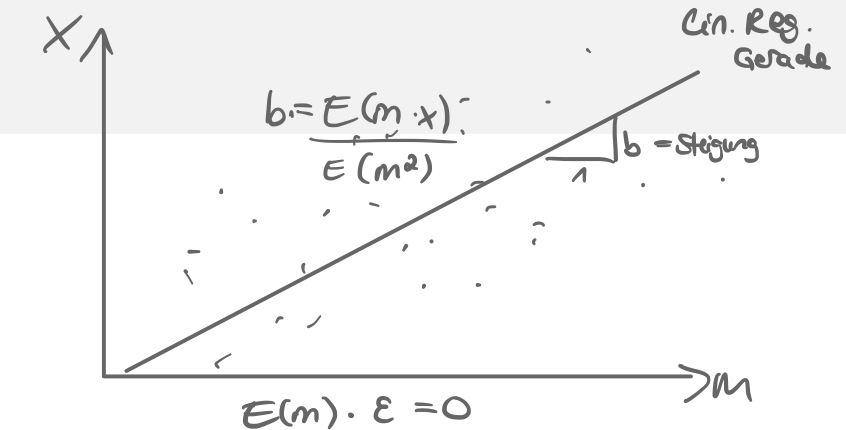
\includegraphics[scale=0.3]{img/p44}
\end{figure*}

\newpage

\section{Beta als Risikomaß}

\textbf{$\beta_i$: Sensitivität der Rendite von Wertpapier $i$ gegenüber der Rendite des ganzen Marktes}
\begin{itemize}
	\item das klassische Risikomaß der Finanzwirtschaft
	\item typischerweise anhand des CAPM  bestimmt
	\item Anwendung als Maß für systematisches Risiko
\end{itemize}
 
\begin{figure*}[h!] \centering
	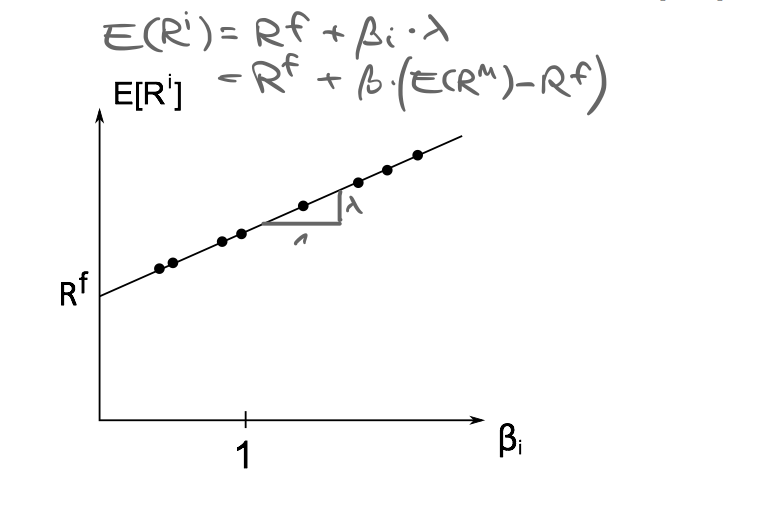
\includegraphics[scale=0.4]{img/p45}
\end{figure*}
Wertpapiermarktlinie (gilt für alle Wertpapiere):
$$ \mathbb{E} \left[ R^i \right] = R^f + \beta_i \cdot \lambda = R^f + \beta_i \cdot \left( \mathbb{E}\left[R^m \right] - R^f \right). $$

Formal: $\beta_i = \frac{\cov(R^i, R^M)}{\operatorname{var}(R^M)}$ mit $R^M$ als Marktrendite. ~\\

Umformung der Return-Beziehung $\mathbb{E}[R^i] = R^f - R^f \cov(m, R^i)$ führt zu

	$$ \mathbb{E}\left[ R^i \right] = R^f + \underbrace{\left( \frac{\cov \left( m, R^i \right)}{\var \left( m \right)} \right)}_{\eqqcolon \beta_{i,m}} \underbrace{\left( - \frac{\var \left( m \right)}{\mathbb{E} \left[ m \right]} \right)}_{\eqqcolon \lambda_{m}},  $$
wobei $\beta_{i,m} =$ normierte Kovarianz (Risikomenge, WP-spezifisch), $\lambda_m$ (nicht WP-spezifisch), mit
\begin{itemize}
	\item $\beta_{i,m} = \frac{\cov \left( m, R^i \right)}{\var \left( m \right)}$ (Risikomenge)
	\item $\lambda_m = - \frac{\var \left( m \right)}{\mathbb{E} \left[ m \right]}$ (Preis des Risikos)
\end{itemize}
$$ \Rightarrow \mathbb{E} \left[ R^i \right] = R^f + \beta_{i, m} \lambda_m $$
CAPM-ähnliche lineare Rendite/Risiko-Beziehung mit
\begin{itemize}
	\item Risikomenge: Normierte Kovarianz mit Diskontfaktor (wertpapierspezifisch)
	\item Preis des Risikos (für alle Assets identisch) abhängig von Volatilität des Diskontfaktors
\end{itemize}

\begin{figure*}[h!] \centering
	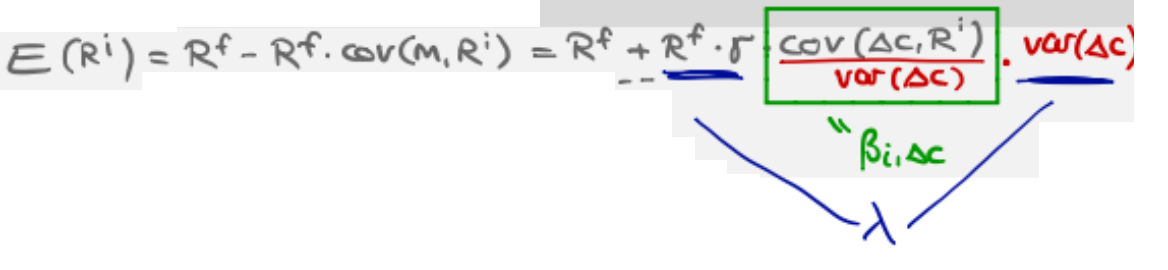
\includegraphics[scale=0.4]{img/p47-1}
\end{figure*}

Betrachte wieder die Approximation für $m$ aus dem Konsummodell (beachte: hier ist das Konsumwachstum $\Delta c_{t+1}$ stochastisch)
	$$ m_{t+1} \approx 1 - \delta - \gamma \Delta c_{t+1} \Rightarrow \mathbb{E} \left[ R^i \right] \approx R^f + \beta_{i, \Delta c} \lambda_c $$
Wieder CAPM-ähnliche lineare Rendite/Risiko-Beziehung mit
\begin{itemize}
	\item Risikomenge: Normierte Kovarianz mit Konsumwachstum (wertpapierspezifisch)
	\item Preis des Risikos $\lambda_c = \frac{\gamma \var \left( \Delta c \right)}{\mathbb{E} \left[ m \right]} = \gamma \var \left( \Delta c \right) R^f$ abhängig von Risikoaversion und Volatilität des Konsums
\end{itemize}
Erwartete Rendite muss umso höher sein,
\begin{itemize}
	\item je riskanter die Zahlung gemessen durch $\beta$
	\item je risikoaverser Akteure sind ($\gamma$) und je riskanter Umfeld ($\var \left( \Delta c \right)$)
\end{itemize}

\begin{figure*}[h!] \centering
	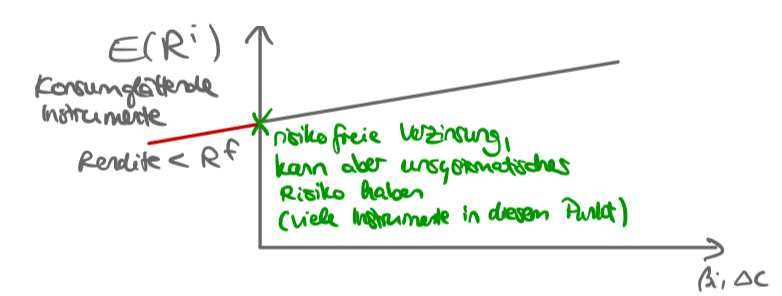
\includegraphics[scale=0.6]{img/p47-2}
\end{figure*}

Je höher $\gamma$ (risikoaverser), desto höher Steigung; je höher Konsumwachstum, desto höher Steigung.

\subsubsection*{Zusammenfassung}

Die Zentrale Bewertungsbeziehung
	$$ p^i = \mathbb{E} \left[ m \cdot x^i \right], $$
für Returns angewendet bedeutet, dass
	$$ 1 = \mathbb{E} \left[ m \cdot R^i \right]. $$
Dies liefert in wenigigen Schritten die lineare Return/Beta-Beziehung bzgl. des Diskontfaktors $m$, mit $\beta_{i, m} = \frac{\cov \left(m, R^i \right)}{\var(m)}$
	$$ \mathbb{E} \left( R^i \right) = R^f + \beta_{i,m} \cdot \lambda_m \quad 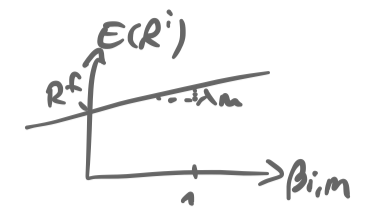
\includegraphics[scale=0.5]{img/p47-3} $$

bzw. (über Approximation von $m$)
$$ \mathbb{E} \left( R^i \right) = R^f + \beta_{i, \Delta c} \cdot \lambda_c \quad 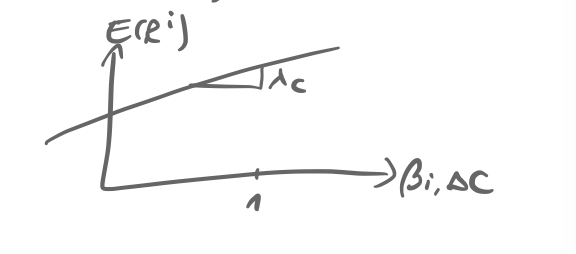
\includegraphics[scale=0.5]{img/p47-4} $$
lineare Return/Beta-Beziehung bzgl des Konsumwachstums $\Delta c$, mit $\beta_{i, \Delta c} = \frac{\cov \left(\Delta c, R^i \right)}{\var(\Delta c)}$
\textbf{keine} Aussage über: was ist handelbar, Nutzenfunktion $\rightarrow$ hier ganz allgemeingültig. CAMP: welche WPs gibt es, Normalverteilung... (viele Annahmen), ABER: empirische Proxies für $\beta_i$ und $m \rightarrow$ Anwendbarkeit!

\newpage

\section{Der $\mu$-$\sigma$-Rand}

Häufig betrachten wir
\begin{itemize}
	\item Erwartungswerte $\mu$ (als Renditemaß)
	\item Varianzen $\sigma^2$ (bzw. $\sigma$ als Risikomaß)
\end{itemize}
der Renditen. Welche Rendite/Risiko-Kombinationen sind überhaupt erreichbar? Für die Rendite $R^i$ gilt ($\rho$ ist die Korrelation):
	$$ 1 = \mathbb{E} \left[ m R^i \right] = \mathbb{E}[m] \mathbb{E} \left[ R^i \right] + \underbrace{\rho_{m, R^i} \sigma(R^i) \sigma(m)}_{\cov(m, R^i)} $$
	$$ \iff R^f = \frac{1}{\mathbb{E}[m]} = \mathbb{E} \left[ R^i \right] + \rho_{m, R^i} \sigma( R^i) \cdot \frac{\rho(m)}{\mathbb{E}[m]} $$
bzw.
	$$ \mathbb{E} \left[ R^i \right] =  R^f  - \rho_{m, R^i} \cdot \sigma( R^i) \cdot \frac{\rho(m)}{\mathbb{E}[m]}. $$
~\\
Da $\rho_{m, R^i} \leq 1$ folgt 
	$$ \left| \mathbb{E} \left[ R^i \right] - R^f \right| \leq \sigma (R^i) \frac{\sigma(m)}{\mathbb{E}[m]} $$
Mittelwert/Standardabweichung-Kombinationen liegen zwingend in kegelförmigem Bereich	

\begin{figure*}[h!] \centering
	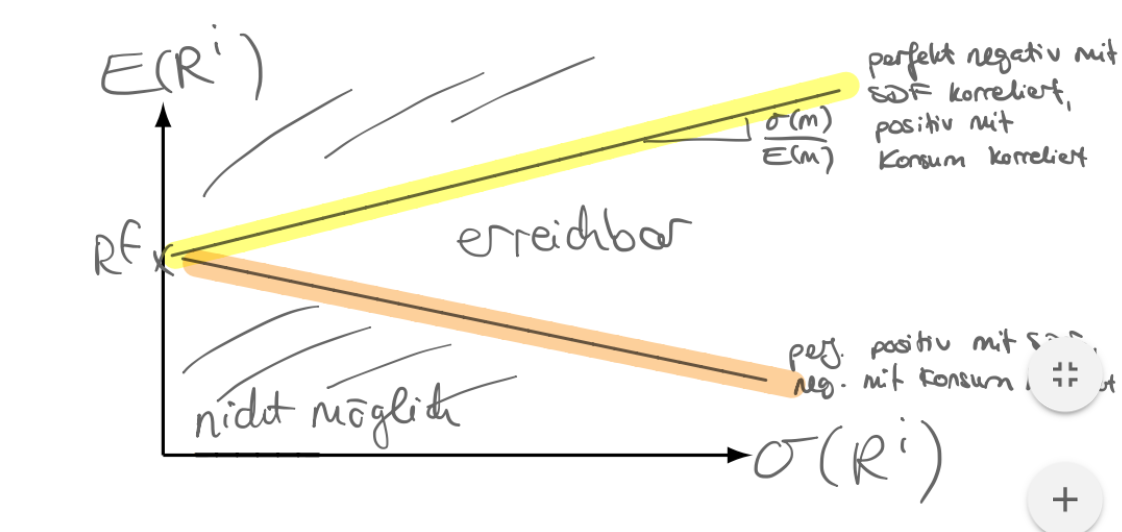
\includegraphics[scale=0.5]{img/p49}
\end{figure*}	
	
Rand der Fläche: wieviel Return ist bei gegebener Volatilität im Mittel möglich? Alle Rand-Returns sind perfekt korreliert mit dem Diskontfaktor $m$
\begin{itemize}
	\item oberer Rand $\rho_{m, R^i} = -1$ bzw. $\rho_{c, R^i} = +1 \Rightarrow$ maximal riskant, maximaler Ertrag
	\item unterer Rand. $\rho_{m, R^i} = +1$ bzw. $\rho_{c, R^i} = -1 \Rightarrow$ bestmögliche Versicherung gegen Konsumschwankungen
\end{itemize}	
Alle Rand-Returns sind perfekt miteinander korreliert. ~\\

Betrachte nun beliebige Return $R^i$. Anstatt $\beta$-Repräsentation
	$$ \mathbb{E}\left[ R^i \right] = R^f + \left( \frac{\cov \left( m, R^i \right)}{\var(m)} \right) \left( - \frac{\var(m)}{\mathbb{E}[m]} \right) = R^f + \beta_{i, m} \lambda_m $$
bezogen auf stochastischen Diskontfaktor. Neue $\beta$-Repräsentation bezogen auf beliebigen (effizienten) Rand-Return $R^{mv}$ ($\neq R^f$) möglich:	
	$$ \mathbb{E} \left[ R^i \right] = R^f + \left( \frac{\cov \left( R^{mv}, R^i \right)}{\var \left( R^{mv} \right)} \right) \left( \mathbb{E} \left[ R^{mv} \right] - R^f \right) = R^f + \beta_{i, mv} \lambda $$
(single-beta Darstellung bzgl. beliebigem effizienten Rand-Return). ~\\

Begründung:
\begin{description}
	\item Schritt 1: Selle stochastischen Diskontfaktor $m$ aus risikolosem Return $R^f$ und beliebigem effizienten Rand-Return $R^{mv}$ dar (Beziehung von $m$ und Rand-Return).
	\item Schritt 2: Setze gefundene Beziehung in ursprüngliche $\beta$-Repräsentation ein und leite daraus neue Darstellung ab:
		$$ \mathbb{E} \left[ R^i \right] = R^f + \beta_{i, mv} \lambda $$
\end{description}
\begin{description}
	\item Ergebnis 1 (wichtig!): Jeder beliebige effiziente Rand-Return $R^{mv}$ ($\neq R^f$) enthält die gesamt Information, die zur Bewertung notwendig ist (genau wie $m$!)
	\item Mittelwert/Standardabweichungs-Kombinationen beliebiger Returns liegen innerhalb des gesamten kegelförmigen Bereichs. Mittelwert/beta-Kombinationen beliebiger Returns liegen auf einer Geraden.
\end{description}
\newpage
\textbf{Formale Ableitung (Schritt 1):} ~\\
Betrachte zunächst die Zahlung $R^m = \frac{m}{\mathbb{E}\left[ m^2 \right]}$
\begin{itemize}
	\item Was ist der Preis $p \left( R^m \right)$?
		$$ p = \mathbb{E} \left[ m \cdot R^m \right] = \mathbb{E} \left[ m \cdot \frac{m}{\mathbb{E} \left[ m^2 \right]} \right] = 1 $$
	\item Wie lässt sich $R^m$ interpretieren? $R^m$ lässt sich als Return interpretieren $\hookrightarrow$ liegt im Kegel.
\end{itemize} 
Konstruiere nun $R^m$ aus risikolosem Return $R^f$ und beliebigem effizienten Rand-Return $R^{mv}$ ($w$: Gewicht):
$$ R^m = w R^f + (1- w) R^{mv} $$
$$ \Rightarrow w = \frac{\mathbb{E} \left[ R^m \right] - \mathbb{E} \left[ R^{mv} \right]}{R^f - \mathbb{E} \left[ R^{mv} \right]}, ~ 1-w = \frac{R^f - \mathbb{E} \left[ R^{m} \right]}{R^f - \mathbb{E} \left[ R^{mv} \right]} $$
~\\
\textbf{Formale Ableitung (Schritt 2):} ~\\
Aus Schritt 1 folgt 
	$$ m = \mathbb{E} \left[ m^2 \right] w R^f + \mathbb{E} \left[ m^2 \right] \left( 1 - w \right) R^{mv} $$
(was eine Beziehung zwischen $m$ und $R^{mv}$ darstellt). Einsetzen in
	$$ \mathbb{E} \left[ R^i \right] = R^f + \left( \frac{\cov \left(m, R^i \right)}{\var \left( m \right)} \right) \left( - \frac{\var(m)}{\mathbb{E} [m]} \right) $$
führt wegen 
\begin{align*}
	\cov \left( m, R^i \right) & = \mathbb{E} \left[ m^2 \right] (1 - w) \cov \left( R^{mv}, R^i \right) \\
	\var (m) & = \left( \mathbb{E} \left[ m^2 \right] \left(1 - w \right) \right)^2 \var \left( R^{mv} \right)
\end{align*}
auf
$$ \mathbb{E} \left[ R^i \right] = R^f + \underbrace{ \left( \frac{\cov \left( R^{mv}, R^i \right)}{ \var \left( R^{mv} \right)} \right)}_{= \beta_{i,mv}} \left( \mathbb{E}\left[ R^{mv} \right] - R^f \right) $$


% Lecture Notes - End 
% todo Lecture-Exercise-Break
% Exercise - Start

\chapter{Übungen}

\subsubsection*{Aufgabe 7}

\begin{enumerate}
	\item Es gilt (vgl. letzte Übung): $m_{t+1} = \beta \frac{u'(c_{t+1})}{u'(c_{t})}$.
		\begin{itemize}
			\item Im schlechten Zustand nimmt der stochastische Diskontfaktor relativ große Werte an (Grenzwert des Konsums ist hoch).
			\item Im guten Zustand relativ geringe Werte.
		\end{itemize}
		Damit ist:
		\begin{align*}
			& m_{t+1} = 0.97 \text{: ungünstiger Zustand} \\
			& m_{t+1} = 0.85 \text{: günstiger Zustand}
		\end{align*}
		\textit{Beachte: \enquote{Im schlechten Zustand} bezieht sich eigentlich relativ auf den Vergleich zu vorhergehenden Periode.}
	\item Eine Power-Nutzenfunktion hat bei uns die allgemeine Form:
		$$ u(c) = \frac{c^{1-\gamma} - 1}{1 - \gamma} $$
		Daraus folgt $u'(c) = c^{-\gamma}$ und damit: % todo -gamma scheint mir im folgenden nicht zu stimmen
		$$ m_{t+1} = \beta \frac{c_{t+1}^{\gamma}}{c_t^{-\gamma}} = \beta \left( \frac{c_t}{c_{t+1}} \right)^\gamma $$
		Ist $\gamma > 0 \Rightarrow$ je größer der Konsum in einem Zustand in $t+1$ ist, desto kleiner $m_{t+1}$ und umgekehrt
	\item $p_A > p_B$ da Wertpapier $A$ im ökonomisch schlechteren Zustand mehr auszahlt und der Erwartungswert der Auszahlung beider Wertpapiere gleich ist.
	\item Es ist
		\begin{align*}
			p_t^A & = \mathbb{E}(m_{t+1} x_{t+1}^A) = 0.5 \cdot 0.85 \cdot 5 + 0.5 \cdot 0.97 \cdot 8 = 6.01 \\
			p_t^B & = analog = 5.83
		\end{align*}
		% todo Zeichnung: Siehe Block
		$\mathbb{E}[R_{t+1}^B] > \mathbb{E}[R_{t+1}^A]$, $p_A > p_B$
	\item Es ist
		\begin{align*}
			p_t & = \mathbb{E}[m_{t+1} X_{t+1}] \\
				& = \mathbb{E}[m_{t+1}] \cdot \mathbb{E}[x_{t+1}] + \cov(m_{t+1}, x_{t+1}) \\
			& = \frac{\mathbb{E}[x_{t+1}]}{R^t} + \cov(m_{t+1}, x_{t+1})
		\end{align*}
		$\Rightarrow \mathbb{E}(x_{t+1}Â) = \mathbb{E}(x_{t+1}^B) = 6.5$
		$$ R^f = \frac{1}{\mathbb{E}(m_{t+1})} = \frac{1}{0.91} = 1.10 $$
		$\Rightarrow \frac{\mathbb{E}(x_{t+1}^A)}{R^f} = \frac{\mathbb{E}(x_{t+1}^B)}{R^f} = 5.91$
		\begin{align*}
			& \cov(m_{t+1}, x_{t+1}) = 0.5 \left( 0.85 - 0.91 \right) \left( 5 - 6.5 \right) + 0.5 \left(0.97 - 0.91 \right) \left( 8 - 6.5 \right) = 0.09 \\
			& \cov(m_{t+1}, x_{t+1}^B) = analog = -0.09 
		\end{align*}
		wobei $\cov(a, b) = \mathbb{E}[(a - \overline{a})(b - \overline{b})]$, mit $\overline{x} = \mathbb{E}[x]$, 
	$$\Rightarrow p^A > p^B$$
	\item Da die $\cov(\cdot, \cdot)$ negative sowie positive Werte annehmen kann, ergibt sich bei geeiegneten Werten für $\mathbb{E}(x_{t+1})$ und $R^f$ für manche Wertpapiere auch bei $\mathbb{E}(x_{t+1}) < 0$ ein positiven Preis. Beispiel: Versicherung
\end{enumerate}

\newpage

\subsubsection*{Aufgabe 8 (Der $\mu$-$\sigma$-Rand)}

Betrachten Sie ein Ökonomie mit zwei Zeitpunkten ($t$ und $t+1$) und einem risikolosen Zinssatz von 10\%.

\begin{enumerate}
	\item Unterstellen Sie für den SDF, das $m_{t+1} = a + b R^{mv}$, wobei $a$ und $b$ Parameterwerte und $R^{mv}$ die Rendite eines Wertpapiers darstellt.
		\begin{enumerate}
			\item Welche Voraussetzung muss erfüllt sein, damit dieser Zusammenhang gelten kann? Welche Implikation für die Bewertung von Wertpapieren enthält diese Annahme.
				\begin{proof}
					Damit der Zusammenhang $m_{t+1} = a + b R^{mv}$ gilt, muss die Rendite des Wertpapiers, $R^{mv}$ perfekt mit $m_{t+1}$ korreliert sein. ~\\
					Das impliziert, dass in $R^{mv}$ alle bewertungsrelevanten Informationen enthalten sein müssen.
				\end{proof}
			\item Maximale Sharpratio und
				\begin{proof}
					$p_{t+1} = \mathbb{E}(m_{t+1} x_{t+1}) \iff 1 = \mathbb{E}(m_{t+1} R_{t+1})$
					\begin{align*}
						& \iff 1 = \mathbb{E}(m_{t+1}) \mathbb{E}(R_{t+1}) + \cov(m_{t+1}, R_{t+1}) \qquad \qquad \qquad \\
						& \iff \mathbb{E}(R_{t+1}) = R^f - \frac{\cov(m_{t+1}, R_{t+1})}{\mathbb{E}(m_{t+1})}  \\
						& \iff \mathbb{E}(R_{t+1}) - R^f = - \rho_{m_{t+1}, R_{t+1}} \sigma_{R_{t+1}} \frac{\sigma_{m_{t+1}}}{\mathbb{E}(m_{t+1})} \\
						& \iff \frac{\mathbb{E}(R_{t+1}) - R^f}{\sigma_{R_{t+1}}} = -\rho_{m_{t+1}, R_{t+1}} \frac{\sigma_{m_{t+1}}}{\mathbb{E}(m_{t+1})} 
					\end{align*}
					
					Mit $|\rho| \leq 1$ gilt:
					$$ \left| \frac{\mathbb{E}(R_{t+1}) - R^f}{\sigma_{R_{t+1}}} \right| \leq \frac{\sigma_{m_{t+1}}}{\mathbb{E}(m_{t+1})}$$
					Aus $m_{t+1} = a + b \cdot R^{mv}_{t+1}$ folgt:
					$$
					  \begin{rcases}
						\operatorname{var}(m_{t+1}) & = b^2 \operatorname{var}(R_{t+1}^{mv}) \\
						\sigma_{m_{t+1}} & = \sqrt{b^2 \operatorname{var}(R_{t+1}^{mv})} = \sqrt{2} \\
						\frac{1}{\mathbb{E}(m_{t+1})}& = R^f = 1.1
					  \end{rcases} \Rightarrow \frac{\sigma_{m_{t+1}}}{\mathbb{E}(m_{t+1})} = 1.55 
					$$
				\end{proof}
		\end{enumerate}
\end{enumerate}

\subsubsection*{Aufgabe 9 (Der $\mu$-$\sigma$-Rand und die Beta-Darstellung)}

Gegeben ist eine Ökonomie mit zwei Zeitpunkten ($t$ und $t+1$) mit einem risikolosen Zinssatz in Höhe von $R^f$, sowie ein effizienter Rand-Return $R^{mv}$. Nehmen Sie an

\begin{enumerate}
	\item Es gilt $m_{t+1} = a + b \cdot R^{mv}$
		\begin{align*}
			p_t & = \mathbb{E}(m_{t+1} x_{t+1}) = \mathbb{E}(m_{t+1}) \mathbb{E}(x_{t+1}) + \cov(m_{t+1}, x_{t+1}) \\
			& \iff p_{t} = \frac{\mathbb{E}(x_{t+1})}{R^f} + \cov(m_{t+1}, x_{t+1}) \\
			& \iff p_{t} = \frac{\mathbb{E}(x_{t+1})}{R^f} + \cov(a + b R^{mv}, x_{t+1})\\
			& \iff p_{t} = \frac{\mathbb{E}(x_{t+1})}{R^f} + b \cov(R^{mv}, x_{t+1})
		\end{align*}
		$\Rightarrow$ falls $b$ bekannt können mit Hilfe von $R^{mv}$ alle Wertpapiere bewertet werden.
	\item Gilt für alle Wertpapiere auf dem $\mu$-$\sigma$-Rand außer dem risikolosen Instrument.
	\item Es gilt die folgenden Möglichkeiten
		\begin{itemize}
			\item 1. Möglichkeit: 
					\begin{align*}
					1 & = \mathbb{E}(m_{t+1} R^{mv}) = \mathbb{E}\left((a + b R^{mv}) R^{mv} \right) \\
					& = \mathbb{E}\left( a R^{mv} + b \left(R^{mv} \right)^2 \right)   \tag*{$(*)$} ~\\
					1 & = \mathbb{E}(m_{t+1} R^{f}) = \mathbb{E}\left((a + b R^{mv}) R^{f} \right) \\
					& = \mathbb{E}\left( a R^{f} + b R^{mv} R^f \right)   \tag*{$(**)$}
				\end{align*}
				Aus $(*)$: $\Rightarrow 1 = a \cdot \mathbb{E}(R^{mv}) + b \mathbb{E}\left(\left(R^{mv} \right)^2 \right)$ ~\\
				Aus $(**)$: $\Rightarrow 1 = a \cdot \mathbb{E}(R^{f}) + b \mathbb{E}\left(\left(R^{f} \right)^2 \right)$
				$$\Rightarrow$$
			\item 2. Möglichkeit: aus $|\rho| = 1$ folgt ($\mathbb{E}(m_{t+1}) = a + b \mathbb{E}(R^{mv})$)
				\begin{align*}
					m_{t+1} & = \mathbb{E}(m_{t+1}) + b \left( R^{mv} - \mathbb{E}(R^{mv}) \right) \tag*{$(+)$} \\
						& \iff m_{t+1} = \frac{1}{R^f} + b \left( R^{mv} - \mathbb{E}(R^{mv}) \right)  \tag*{$(***)$}
				\end{align*}
				Außerdem: $1 = \mathbb{E}(m_{t+1} E^{mv}$. Daraus folgt indem wir $(***)$ einsetzen:
					\begin{align*}
						1 & = \mathbb{E} \left[ \left( \frac{1}{R^f} + b \left( R^{mv} - \mathbb{E}_t \left( R^{mv} \right) \right) \right) R^{mv} \right] \\
						& \iff 1 = \frac{1}{R^f} \mathbb{E}(R^{mv}) + b \mathbb{E}\left( \left((R^{mv} \right)^2 \right) - b \mathbb{E} \left(R^{mv} \right)^2 \\
						& \iff 1 = \frac{1}{R^f} \mathbb{E}(R^{mv}) + b \operatorname{var}(R^{mv}) \\
						& \iff b = - \frac{\mathbb{E}(R^{mv}) - R^f}{R^f \operatorname{var}(R^{mv})}
					\end{align*} 
					In $(+)$ einsetzen:
					\begin{align*}
						m_{t+1} & = \mathbb{E}(m_{t+1}) + \left( - \frac{\mathbb{E}(R^{mv}) - R^f}{R^f \operatorname{var}(R^{mv})} \right) \left( R^{mv} - \mathbb{E}(R^{mv} \right) \\
						& \iff m_{t+1} = \underbrace{\frac{1}{R^f} + \mathbb{E}(R^{mv}) \frac{\mathbb{E}(R^{mv} - R^f}{R^f \operatorname{var}(R^{mv})}}_{\eqqcolon a} \underbrace{- \frac{\mathbb{E}(R^{mv}) - R^f}{R^f \operatorname{var}(R^{mv})}}_{\eqqcolon b} R^{mv} \tag*{$(++)$} \\
						& \iff m_{t+1} = a + b R^{mv}
					\end{align*} 
		\end{itemize}
		\item Beta Darstellung
			$$ p_{t} = \mathbb{E}(m_{t+1} x_{t+1}) \iff 1 = \mathbb{E}(m_{t+1}) \mathbb{E}(R^i_{t+1}) + \cov(m_{t+1}, R^i_{t+1}) $$
			$$ \mathbb{E}(R_{t+1}^i) = R^f - \frac{\cov(m_{t+1}, R_{t+1}^i)}{\mathbb{E}(m_{t+1})} $$
			Aus $(++)$ folgt
			$$ \mathbb{E}(R_{t+1}^i) = R^f + \frac{\mathbb{E}(R^{mv} - R^f)}{R^f \operatorname{var}(R^{mv})} \cov(R^{mv}, R_{t+1}^i) \frac{1}{\mathbb{E}(m_{t+1})} $$
			$$ \iff \mathbb{E}(R_{t+1}^i) = \R^f + \frac{\mathbb{E}(R^{mv} - R^f}{\operatorname{var}(R^{mv}} \cov(R^{mv}, R^i) $$
			$$ \iff \mathbb{E}(R^i_{t+1}) = R^{f} + \underbrace{\frac{\cov(R^{mv}, R^{i}_{t+1})}{\operatorname{var}(R^{mv})}}_{\eqqcolon \beta_{i, mv}} \underbrace{\left( \mathbb{E}(R^{mv} - R^f \right)}_{\eqqcolon \lambda_{mv}} $$
			$$ \iff \mathbb{E}(R^i_{t+1}) = R^f + \beta_{i, mv} \lambda_{mv} $$
		\item Welche Annahme trift man oft in der parktischen Umsetzung dieser Bewertungsbeziehung
			\begin{proof}
				$R^{mv} =$ Rendite des Marktportfolios (z.B. Dax 30)
			\end{proof}
\end{enumerate}

\newpage

\subsection*{Sonderübung}

\subsubsection*{Aufgabe 1}
Nehmen Sie Stellung zu folgenden Aussagen:
\begin{enumerate}
	\item Wertpapiere, deren Auszahlung positiv mit dem stochastischem Diskontfaktor  korrelieren, besitzen im Gleichgewicht höhere erwartete Renditen, die für das höhere Risiko solcher Wertpapiere kompensieren.
		\begin{proof}
			Die Aussage ist falsch. Wertpapiere deren erwarteten. Renditen positiv mit dem stoch. Diskontfaktor korrelieren, zahlen in Zuständen mit hohem stoch. Diskontfaktor wenig und in Zuständen mit niedrigem stoch. Disktontfaktor viel (es ist ja: SDF hoch = schlechter Zustand und vice versa). Solch ein Wertpapier besitzt einen Versicherungscharakter. Wichtig ist, dass die Renditen-Preisbeziehung invers ist. Im Gleichgewicht beizten sie also niedrige erwartete Renditen, da sie ein geringeres Risiko besitzen.
		\end{proof}
	\item Wertpapiere, die nicht auf dem $\mu$-$\sigma$-Rand liegen, sind nicht effizient und werden deshalb von den Investoren nicht nachgefragt.
		\begin{proof}
			Die Aussage ist falsch. Diese Wertpapiere sind nicht effizient, allerdings sind sie auch nicht perfekt mit stochastischen Diskontfaktor korreliert und weisen unsystematisches Risiko auf. Damit können diese Wertpapiere nachgefragt werden, jedoch nicht alleine.
		\end{proof}
	\item Das CAPM kann nicht stimmen, da tatsächlich die Korrelation von zukünftigen Zahlung mit dem Konsumwachstum entscheidend für den Preis eines Wertpapiers ist nachgefragt.
		\begin{proof}
			Diese Aussage ist falsch. CAMP ist ein Spezialfall des konsumbasierten Asset Pricing Modells. Als Faktormodell nutzt das CAMP eine Approximation des aggregieren Nutzenwacstums
			$$ m_{t+1} = \beta \frac{u'(c_{t+1})}{u'(c_{t})} = a + b' f_{t+1}. $$ 
			Das CAMP-Modell approximiert also diesen Faktor linear und  stellt damit (vereinfacht) die Korrelation dar.
		\end{proof}
	\item Existiert in einer Ökonomie mindestens für jeden Zustand ein Wertpapier, das $24$ im entsprechenden Zustand und $0$ in allen anderen Zuständen auszahlt, so ist auch die Verteilung des stochastischen Diskontfaktors bekannt und alle anderen Wertpapiere können basierend darauf bewertet werden.
		\begin{proof}
			Diese Aussage ist falsch. Obwohl die Auszahlungsmatrix linear unabhängig ist, reicht diese nicht zur Bestimmung der Verteilung des stoch. Diskontfaktors aus und somit können nicht nicht alle weiteren Wertpapiere darauf bewertet werden. Vgl.
			$$ p(x) = \sum_{s \in S} \pi(s) m(s) x(s) $$
			Somit ist der Preis und Eintrittswahrscheinlichkeit müssen gegeben sein.
		\end{proof}
	\item  Da die Zentralbank den Zinssatz festlegt, muss bei der empirischen Anwendung des konsumbasierten Ansatzes stets davon ausgegangen werden, dass der Preis des risikolosen Instruments exogen festgelegt wird. Die Diskussion inwiefern sich die Zinsen z.B. in Folge von geänderter Risikoaversion der Investoren ändern, ist deshalb lediglich exemplarischer Natur und nicht mit der Empirie vereinbar. 
		\begin{proof}
			Nur teilweise richtig. Wechselwirkung zwischen Konsum \% Zinsen
				$$ \Rightarrow \text{ Makro-Sicht } \Rightarrow \text{ Perspektive einer Einzelperson } $$
				Zentralbank setzt zwar Leitzins fest und kauft Anleihen, allerdings gibt es noch andere Einflüsse. ~\\
			$\Rightarrow$ Preis für risikoloses Instrument kann empirisch nicht als exogen gegeben angenommen werden.
		\end{proof}
\end{enumerate}

\newpage

\subsection*{Aufgabe 2}
Gehen Sie von einer Ökonomie mit den Zeitpunkten $t = 0$, $t = 1$ und $t = 2$ ($t$ in Jahren) aus. Die Zustandsübergänge und die Entwicklung des Konsums des repräsentativen Investors sind gemäß dem Baumdiagramm in der Aufgabe zu entnehmen. Der Nutzen des repräsentativen Investors zum jeweiligen Zeitpunkt t lässt sich mit Hilfe der folgenden Powernutzenfunktion mit $\gamma = 1.5$ quantifizieren:

$$ u(c_t) = \frac{c_t^{1-\gamma}}{1 - \gamma} $$

Nehmen Sie für die zeitliche Diskontierung $\beta = 0.95$ an.
\begin{enumerate}
	\item Für die Zustandsübergangswahrscheinlichkeiten gilt zunächst $p_1 = p_{21} = p_{22} = 0.5$. Bestimmen Sie die beiden fairen risikolosen Zinssätze (annualisiert) für die Zeiträume $t = 0$ bis $t = 1$ und $t = 0$ bis $t = 2$. Berechnen Sie außerdem den erwarteten Gesamtnutzen des repräsentativen Investors zum Zeitpunkt $t = 0$.
		\begin{proof}
		Es ist $u'(c_t) = c_t^{-\gamma}$ und damit (vgl. Cochrane, S. 24f)
		$$ R_{t+1}^f = \frac{1}{\mathbb{E}\left[ \beta \frac{u'(c_{t+1})}{u'(c_t)} \right]} = \frac{1}{\mathbb{E}\left[ \beta \left( \frac{c_{t}}{c_{t+1}} \right)^\gamma \right]} $$
		Damit ist
			\begin{align*}
				R_{t+1}^f & = \frac{1}{\mathbb{E}\left[ \beta \left( \frac{c_{t}}{c_{t+1}} \right)^\gamma \right]} \\
				& =\frac{1}{0.5 \cdot 0.95  \left( \frac{20}{25} \right)^{1.5} + 0.5 \cdot 0.95  \left( \frac{20}{21} \right)^{1.5} } \\
				& = 1.2798 ~ \hat{=} ~ 27.98\% \\
			\end{align*}
			\begin{align*}
				R_{t+2}^f & = \frac{1}{\mathbb{E}[m_{0,2}]} = \frac{1}{\mathbb{E}[m_{0,1} \cdot m_{1,2}]}  \\
				& = \frac{1}{\mathbb{E}\left[\beta \cdot \frac{u'(c_1)}{u'(c_0)} \cdot \beta \cdot \frac{u'(c_2)}{u'(c_1)} \right]} \\
				& = \frac{1}{\mathbb{E}\left[ \beta^2 \left( \frac{c_{t}}{c_{t+2}} \right)^\gamma \right]} \\
			& =\frac{1}{0.25 \cdot 0.95^2 \left( \left( \frac{20}{30} \right)^{1.5} +  \left( \frac{20}{26} \right)^{1.5} + \left( \frac{20}{26} \right)^{1.5} + \left( \frac{20}{22} \right)^{1.5} \right)} \\
			& = 1.6056~ \hat{=} ~60.56\%
			\end{align*}
			Damit liegt das Annulalisierte bei $r^f = \sqrt{R_{t+2}^f} = \sqrt{~60.56} = 26.61\%$. Der erwartete Nutzen ergibt sich zu
			\begin{align*}
				U_t(c_t, c_{t+1}, c_{t+2}) & = u(c_t) + \beta \mathbb{E}[ u(c_{t+1})] + \beta^2 \mathbb{E}_t \left[ u(c_{t+2}) \right] \\
						& = -2 \left( \frac{1}{\sqrt{20}} + 0.95 \left( 0.5 \cdot \frac{1}{\sqrt{25}} + 0.5 \cdot \frac{1}{\sqrt{21}} \right)\right) \\
						& \quad-2 \left( 0.95^2 \left( 0.25 \cdot \frac{1}{\sqrt{30}} + 0.25 \cdot \frac{1}{\sqrt{26}} + 0.25 \cdot \frac{1}{\sqrt{26}} + 0.25 \cdot \frac{1}{\sqrt{22}} \right)  \right) \\
						& = - 1.2001
			\end{align*} 
		\end{proof}
	\item Nehmen Sie nun an, dass für die Zustandsübergangswahrscheinlichkeiten $p_1 = 0.5$, $p_{21} = 0.7$ und $p_{22} = 0.3$ gilt. Würde der repräsentative Investor diese Situation der Situation aus Aufgabenteil a) vorziehen? Antworten Sie sowohl mit einer ökonomischen Argumentation als auch mit einer Rechnung.
		\begin{proof}
			Vergleiche den Gesamtnutzen des Investors zwischen a) und b)
				\begin{align*}
				U_t(c_t, c_{t+1}, c_{t+2}) & = u(c_t) + \beta \mathbb{E}[ u(c_{t+1})] + \beta^2 \mathbb{E}_t \left[ u(c_{t+2}) \right] \\
						& = -2 \left( \frac{1}{\sqrt{20}} + 0.95 \left( 0.5 \cdot \frac{1}{\sqrt{25}} + 0.5 \cdot \frac{1}{\sqrt{21}} \right)\right) \\
						& \quad-2 \left( 0.95^2 \left( 0.5 \cdot 0.7 \cdot \frac{1}{\sqrt{30}} + 0.5 \cdot 0.3 \cdot \frac{1}{\sqrt{26}} + 0.5 \cdot 0.3 \cdot \frac{1}{\sqrt{26}} + 0.5 \cdot 0.7 \cdot \frac{1}{\sqrt{22}} \right)  \right) \\
						& = - 1.2007 < -1.2001
			\end{align*} 		
			Nutzen in $t = 2$ ist volatiler (den Wahrscheinlichkeit bei 30 und 22 zu Lasten). Investoren bevorzugen allerdings einen konstanten Konsum
			$$ \gamma = 1.4 \Rightarrow \text{ risikoavers} $$
			$\Rightarrow$ ziehe a) vor.
		\end{proof}
	\item Welche Auswirkung hätte eine Veränderung der Zustandsübergangswahrscheinlichkeiten gemäß Aufgabenteil b) (im Vgl. zu Aufgabenteil a)) auf den risikolosen Zinssatz von t = 0 bis t = 2? Antworten Sie ohne Rechnung und gehen Sie insbesondere darauf ein, über welchen Kanal (erwarteter Konsumwachstum vs. Volatilität des Konsumwachstums) sich die veränderten Übergangswahrscheinlichkeiten auf den Zinssatz in diesem Fall auswirken.
		\begin{proof}
			Durch die Änderung der Wahrscheinlichkeiten in b) ändert sich der Erwartungswert des Konsums und damit Erwartungswert von $\Delta c_2$ nicht. Was sich geändert hat, ist die Volatilität des Konsumwachstums. Der zukünftige Zustand ist nun unsicher, wodurch man vorzüglich spart (precautionary savings). Durch diese Tatsache erhöht sich die Nachfrage und im Zuge dessen reduzieren sich die Zinsen.
		\end{proof}
	\item Können die risikoneutralen Wahrscheinlichkeiten in der gegebenen Ökonomie berechnet werden? Gehen Sie bei der Beantwortung der Frage darauf ein, wie sich die gegebene Situation im Vergleich zu den Standardsituationen, im Rahmen derer risikoneutrale Wahrscheinlichkeiten in Vorlesung und Übung bestimmt wurden, unterscheidet.
		\begin{proof}
			Rein theoretisch könnten die risikoneutralen Wahrscheinlichkeit für beide Stufen anhand der Formel berechnet werden.
			$$ \pi^*(s) = \frac{m(s)}{\mathbb{E}[m]} \cdot \pi(s) = R^f \cdot pc(s) = R^f \cdot m(s) \cdot \pi(s) $$
			wobei $R^f = R^f_{01}/R_{02,}^f$ und $m(s) = \beta \cdot \frac{u'(c(s))}{u'(c_0)}$ bzw. $m(s)= \beta ^2\cdot \frac{u'(c(s))}{u'(c_0)}$. ~\\
			\textbf{Unterschiede}:
			\begin{itemize}
				\item Es liegt ein zweistufiges Modell vor
				\item In der vorliegenden Situation liegen keinerlei Informationen über Wertpapiere vor (Preis, Auszahlungsprofil, $\dotsc$). ~\\
					Lediglich die Konsumniveaus sind bekannt. ~\\
					Risikoneutrale Wahrscheinlichkeiten im Zusammenhang mit Derivatenbewertung
			\end{itemize} 
			Bemerkung: würde man hier risikoneutrale Wahrscheinlichkeiten berechnen? Nein, da hier einfach Erwartungsnutzen ausgerechnet werden kann $\Rightarrow$ Vorteil risikoneutrale Wahrscheinlichkeiten $\Rightarrow$ keine Aussage über Nutzenfunktion notwendig (diese ist in Aufgabe 2 atypischerweise gegeben).
		\end{proof}
	\item Beschreiben Sie rein qualitativ wie sich die risikoneutralen Wahrscheinlichkeiten $p_1^*$, $p_{21}^*$ und $p_{22}^*$ im Vergleich zu ihren physischen Äquivalenten verhalten. Gehen Sie darauf ein wie die Unterschiede zwischen physischen und risikoneutralen Wahrscheinlichkeiten interpretiert werden können.
		\begin{proof} 
			Es gilt:
			$$ \pi^*(s) = \frac{m(s)}{\mathbb{E}[m] }\cdot m(s) $$
			Die risikoneutralen Wahrscheinlichkeiten sind dann besonders hoch, wenn der Zustand schlecht ist ($m(s)$ ist groß) oder sehr wahrscheinlich ist, d.h. $\pi(s)$ ist groß.
		\end{proof}
\end{enumerate}

% Index									
\renewcommand{\indexname}{Stichwortverzeichnis}
\printindex


\end{document}